\ifdefined \buildingFullOPALManual \else


%\ifx \@buildingFullOPALManual \@empty
%\else

%\documentclass[12pt,a4paper]{report}
\documentclass[a4paper]{book}

%% does not work in Latex2Html mode
%\usepackage{hyperref}

\usepackage[T1]{fontenc}
\usepackage{url}
\usepackage{html}
\usepackage{epic}
\usepackage{eepic}
\usepackage{makeidx}
\usepackage{array}
\usepackage{times}
\usepackage{amsmath}
\usepackage{amsxtra}
\usepackage{bm}
\usepackage[thin,thinp,thinc]{esdiff}
\usepackage{graphicx}
\usepackage{dingbat}
\usepackage{color}
\usepackage{subfig}
\usepackage{boxedminipage}
\usepackage{alltt}
\usepackage{nicefrac}
\usepackage{calc}
%\usepackage{pdfdraftcopy}             % Draft
\usepackage{tikz}
\usetikzlibrary{
  er,3d,calc,fadings,trees,positioning,arrows,chains,decorations.pathreplacing,
  decorations.pathmorphing,shapes,shapes.symbols,shapes.arrows,matrix,through,decorations.text
}

\tikzset{
  >=stealth',
  punktchain/.style={rectangle,rounded corners, draw=black, very thick,text width=10em,
                     minimum height=3em, text centered, on chain},
  line/.style={draw, thick, <-},
  element/.style={tape,top color=white,bottom color=blue!50!black!60!,minimum width=8em,
                  draw=blue!40!black!90, very thick,text width=10em, minimum height=3.5em,
                  text centered, on chain},
  every join/.style={->, thick,shorten >=1pt},
  tuborg/.style={decorate},
  tubnode/.style={midway, right=2pt}
}

\tikzstyle{material}=[draw, fill=blue!20, text width=16.0em, text centered, minimum height=1.5em]
\tikzstyle{diagramstep} = [material, text width=20em, minimum width=10em, minimum height=3em, rounded corners]
\tikzstyle{line} = [draw, thick, color=black!50, -latex']

\usepackage{booktabs}
\usepackage{xspace}
\usepackage{xstring}

\usepackage{fancyvrb}
\usepackage{rotating}
\usepackage{float}

\usepackage{tabularx}
\usepackage{longtable}
\setcounter{LTchunksize}{3}

\usepackage[section]{placeins}
\usepackage{MnSymbol}
\usepackage{microtype}
\usepackage{setspace}
\usepackage{dcolumn}

\usepackage[vmargin={3.0cm,3.0cm},
            hmargin={2.0cm,3.0cm}]{geometry}

\usepackage{upgreek}
\usepackage[binary-units=true]{siunitx}
\sisetup{exponent-product = \cdot,math-ohm=\Upomega,text-ohm=\ensuremath{\Upomega}}
\DeclareSIUnit{\clight}{c}
\DeclareSIUnit\gauss{Ga}

\usepackage{engord}
\usepackage{wasysym}
\DeclareSIUnit[number-unit-product = \,]{\permill}{\permil}

\usepackage{hyperref}
\hypersetup{
    pdftitle          = The OPAL Framework,
    pdfauthor         = {Andreas Adelmann, Achim Gsell, Valeria Rizzoglio, Christof Metzger-Kraus,
                         Yves Ineichen, Xiaoying Pang, Steve Russell, Chuan Wang, Jianjun Yang,
                         Suzanne Sheehy, Chris Rogers, Daniel Winklehner},
    pdfsubject        = User's Reference Manual,
    pdffitwindow      = true,               % page fit to window when opened
    pdfnewwindow      = true,               % links in new window
    colorlinks        = true,               % false: boxed links; true: colored links
    linkcolor         = black!80!green,     % color of internal links
    citecolor         = black!20!red,       % color of links to bibliography
    urlcolor          = blue,               % color of external links
    breaklinks        = true,
    bookmarksnumbered = true,
    plainpages        = false
}

\usepackage{ifthen}

\newif \iflinuxwindows
\linuxwindowstrue   % set this to true when building the manual on Linux or Windows
\iflinuxwindows
\usepackage{epstopdf}
\fi

\usepackage[backend=biber,
            style=phys,
            biblabel=brackets,
            maxnames=3,
            doi=true,
            isbn=true,
            url=true]{biblatex}
%---- macros ----

\renewcommand{\topfraction}{1.0}
\renewcommand{\bottomfraction}{1.0}
\renewcommand{\textfraction}{0.0}
\renewcommand{\arraystretch}{2.0}
\newenvironment{tex2html_nowrap}{}{}


\newcommand{\Newline}{\hfil \\}


\newsavebox{\ExampleBox}
\newenvironment{example}
 {\VerbatimEnvironment
  \begin{flushleft}
  \begin{lrbox}{\ExampleBox}
    \begin{minipage}{\linewidth}
  \begin{Verbatim}[frame=lines,xleftmargin=0cm,fontsize=\footnotesize,samepage=true]}
 {\end{Verbatim}
  \end{minipage}
  \end{lrbox}
  \mbox{\usebox{\ExampleBox}}
  \end{flushleft}
 }

\newenvironment{longexample}
{\Verbatim[frame=lines,xleftmargin=0mm,fontsize=\footnotesize]}
{\endVerbatim}

%\examplefromfile{filename} reads in a text file and displays it in the document.
\newcommand{\examplefromfile}[1]{
\VerbatimInput[frame=lines,xleftmargin=0mm,fontsize=\footnotesize,label=\texttt{#1}]{#1}}

%for upright d of differentials
\makeatletter
\newcount\my@repeat@count

\newcommand{\myrepeat}[2]{%
  \begingroup
  \my@repeat@count=\z@
  \@whilenum\my@repeat@count<#1\do{#2\advance\my@repeat@count\@ne}%
  \endgroup
}

\newcommand{\differential}[1]{\ifstrempty{#1}{\ES@dop\ES@difint}{\ES@dop^{#1}\ES@difint}}
\newcommand{\pdifferential}[1]{\ifstrempty{#1}{{\partial\,}}{{\partial^{#1}\,}}}

\makeatother

\newcommand{\der}[3][]{\frac{\differential{#1}#2}{\differential{}\ifstrempty{#1}{#3}{#3^#1}}}
\newcommand{\parder}[3][]{\frac{\pdifferential{#1}#2}{\pdifferential{}\ifstrempty{#1}{#3}{#3^#1}}}
\newcommand{\niceder}[3][]{\nicefrac{\differential{#1}#2}{\differential{}\ifstrempty{#1}{#3}{#3^#1}}}
\newcommand{\uglyder}[3][]{{\differential{#1}#2}/{\differential{}\ifstrempty{#1}{#3}{#3^#1}}}
\newcommand{\uglyparder}[3][]{{\pdifferential{#1}#2}/{\pdifferential{}\ifstrempty{#1}{#3}{#3^#1}}}
\newcommand{\dd}[1][]{\; \differential{#1}}
\newcommand{\primed}{^{\prime}}
\newcommand{\dprimed}{^{\prime\prime}}
\newcommand{\nprimed}[1]{^{\myrepeat{#1}{\prime}}}

%Editing Macros
\newcommand{\TODO}[1]{{\color{red}\ifthenelse{\boolean{ShowDebug}}{[TODO: #1]}{}}}



%text in gray box
\newsavebox{\fmbox}
\definecolor{lightgray}{gray}{0.95}
\newenvironment{fmpage}
   {\vspace{-1.0cm}\begin{lrbox}{\fmbox}\begin{minipage}[t]{13.5cm}\vspace{0.1cm}}
   {\vspace{-0.4cm}\end{minipage}\end{lrbox}\begin{center}\fcolorbox{black}{lightgray}{\usebox{\fmbox}}\end{center}}


% Definition new signes
\newcommand{\R}{{\mathbb R}} % real numbers
\newcommand{\Q}{{\mathbb Q}} % rational numbers
\newcommand{\Z}{{\mathbb Z}} % integer numbers
\newcommand{\N}{{\mathbb N}} % natural numbers

\newcommand{\mad}{\textsc{mad}\xspace}
\newcommand{\madnine}{\textsc{mad9}\xspace}
\newcommand{\madninep}{\textsc{mad9p}\xspace}
\newcommand{\madeight}{\textsc{mad8}\xspace}
\newcommand{\classic}{\textsc{classic}\xspace}

\makeatletter
\newcommand{\opal@impl}{\textsc{Opal}}
\newcommand{\opalt@impl}{\textsc{Opal-t}}
\newcommand{\opalcycl@impl}{\textsc{Opal-cycl}}
\newcommand{\opalmap@impl}{\textsc{Opal-map}}
\newcommand{\opalenv@impl}{\textsc{Opal-e}}

\newcommand{\opal}{\opal@impl\xspace}
\newcommand{\opalt}{\opalt@impl\xspace}
\newcommand{\opalcycl}{\opalcycl@impl\xspace}
\newcommand{\opalmap}{\opalmap@impl\xspace}
\newcommand{\opalenv}{\opalenv@impl\xspace}

\newcommand{\noopalt}{\leftthumbsdown \opalt@impl\xspace}
\newcommand{\noopalcycl}{\leftthumbsdown \opalcycl@impl\xspace}
\newcommand{\noopalmap}{\leftthumbsdown \opalmap@impl\xspace}
\newcommand{\noopalenv}{\leftthumbsdown \opalenv@impl\xspace}
\makeatother

\newcommand{\impactt}{\textsc{Impact-t}\xspace}
\newcommand{\partroot}{\textsc{H5root}}


\newcommand{\latermore}{More details will be given in Version 1.6.0}


\newcommand{\lieop}[1]{{:}{#1}{:}}

\newcommand{\rms}[1]{\overset{\sim}{#1}}

\newcommand{\sprod}{\cdot}
\newcommand{\vprod}{\times}
\newcommand{\matr}[1]{\mathcal{#1}}
\renewcommand{\vec}[1]{{\bm{#1}}}
\newcommand{\transpose}[1]{#1^\intercal}
\renewcommand{\epsilon}{\varepsilon}

\newcommand{\keyword}[2][]{\ifstrempty{#1}{\texttt{\expandafter\MakeUppercase\expandafter{#2}}}{\hyperref[#1]{\texttt{\expandafter\MakeUppercase\expandafter{#2}}}}}
\newcommand{\tabline}[3][]{\keyword[#1]{#2}& #3 \\}
\newcommand{\tabheadcell}[1]{{\bfseries #1}}

\newcommand*\kdescriptionlabel[1]{\hspace\labelsep
                                \normalfont\keyword{#1}\index{#1}}
\makeatletter
\newenvironment{kdescription}
               {\list{}{\labelwidth\z@ \itemindent-\leftmargin
                        \let\makelabel\kdescriptionlabel}}
               {\endlist}
\makeatother

\ExplSyntaxOn
\NewDocumentCommand{\tabhead}{ m }
 {
  \seq_set_split:Nnn \l_tmpa_seq { & } { #1 }
  \bfseries \seq_use:Nn \l_tmpa_seq { & \bfseries } \\
 }

\NewDocumentCommand \multrefImpl { O{ } m m m } {
  \ifnumgreater{\clist_count:n {#4}}{1}{
    \seq_set_from_clist:Nn \l_tmpa_seq { #4 }

    \seq_set_map:NNn \l_tmpb_seq \l_tmpa_seq { \exp_not:n { \ref{#3:##1} } }
    \ifstrempty{#1}{#2s}{#1}~\seq_use:Nnnn \l_tmpb_seq {\ and\ } {,\ } {,\ and\ }
  }{
    #2~\ref{#3:#4}
  }
}

\NewDocumentCommand \multeqnrefImpl { m } {
  \ifnumgreater{\clist_count:n {#1}}{1}{
    \seq_set_from_clist:Nn \l_tmpa_seq { #1 }

    \seq_set_map:NNn \l_tmpb_seq \l_tmpa_seq { \exp_not:n { \eqref{eq:##1} } }
    Equations~\seq_use:Nnnn \l_tmpb_seq {\ and\ } {,\ } {,\ and\ }
  }{
    Equation~\eqref{eq:#1}
  }
}
\ExplSyntaxOff


%Abbreviations for Equations, Figures, and Tables
%\newcommand{\Equation}[1]{Equation~\eqref{#1}}

\newcommand{\bibref}[2]{#1 \cite{bib:#2}}
\newcommand{\figref}[1]{\multrefImpl{Figure}{fig}{#1}}
\newcommand{\chpref}[1]{\multrefImpl{Chapter}{chp}{#1}}
\newcommand{\appref}[1]{\multrefImpl[Appendices]{Appendix}{chp}{#1}}
\newcommand{\secref}[1]{\multrefImpl{Section}{sec}{#1}}
\newcommand{\ssecref}[1]{\multrefImpl{Section}{ssec}{#1}}
\newcommand{\tabref}[1]{\multrefImpl{Table}{tab}{#1}}
\newcommand{\eqnref}[1]{\multeqnrefImpl{#1}}

\newcommand{\seefig}[1]{(see~\figref{#1})}
\newcommand{\seechp}[1]{(see~\chpref{#1})}
\newcommand{\seesec}[1]{(see~\secref{#1})}
\newcommand{\seessec}[1]{(see~\ssecref{#1})}
\newcommand{\seetab}[1]{(see~\tabref{#1})}
\newcommand{\seeeqn}[1]{(see~\eqnref{#1})}

\newcommand{\filename}[1]{\emph{#1}}


% Define distances for bordering
\newcommand{\blockdist}{1.3}
\newcommand{\edgedist}{1.5}
\newcommand{\diagramstep}[2]{node (p#1) [diagramstep] {#2}}


% place chapter title page on odd pages
\let\stdchapter\chapter
\makeatletter
\renewcommand*{\chapter}{\if@openright\cleardoublepage\else\clearpage\fi\stdchapter}

\makeatother

\IfFileExists{./version.tex}{%
  \newcommand{\opalversion}[1]{Version \ifstrempty{#1}{1.9.0}{#1}\xspace}
%
}%
{%
  \newcommand{\opalversion}[1]{\ifstrempty{#1}{current Version}{Version #1}\xspace}%
}
\newboolean{ShowMap}
\setboolean{ShowMap}{false}

\newboolean{ShowEnv}
\setboolean{ShowEnv}{false}

\newboolean{ShowDebug}
\setboolean{ShowDebug}{false}

%----Control Structures
\newboolean{FullOPALManual}
\setboolean{FullOPALManual}{false}


\makeindex


\bibliography{bibliography}
\begin{document}

\fi
\chapter{Benchmarks}
\label{chp:benchmarks}

\section{\opalt compared with TRANSPORT \& TRACE 3D}
\label{sec:T3D}

\subsection{TRACE 3D}
TRACE 3D is an interactive beam dynamics program that calculates the envelopes of a bunched beam, including linear space-change forces  \cite{Trace_man}. It provides an instantaneous beam profile diagram and delineates the transverse and longitudinal phase plane, where the ellipses are characterized by the Twiss parameters and emittances (total and unnormalized).

\subsection{TRACE 3D Units}
\label{ssec:T3D_units}

TRACE 3D supports the following internal coordinates and units for the three phase planes:

\begin{itemize}
\item \textbf{horizontal plane:} \\
x [mm] is the displacement from the center of the beam bunch;\\
x' [mrad] is the beam divergence;

\item \textbf{vertical plane:}\\
y [mm] is the displacement from the center of the beam bunch; \\
y' [mrad] is the beam divergence;

\item \textbf{longitudinal plane:}\\
z [mm] is the displacement from the center of the beam bunch; \\
$\Delta$p/p [mrad] is the difference between the particle's longitudinal momentum and the reference momentum of the beam bunch.
\end{itemize}

For input and output, however, z and $\Delta$p/p are replaced by $\Delta\phi$ [degree] and $\Delta$W [keV], respectively the displacement in phase and energy. The relationships between these longitudinal coordinates are:

\begin{equation}
z = -\frac{\beta\lambda}{360}\Delta\phi
\end{equation}
and
\begin{equation}
\frac{\Delta p}{p} = \frac{\gamma}{\gamma +1}\frac{\Delta W}{W}
\end{equation}
where $\beta$ and $\gamma$ are the relativist parameters, $\lambda$ is the free-space wavelength of the RF and W is the kinetic energy [\si{\mega\electronvolt}] at the beam center. This internal conversion can be displayed using the \textit{command W} (see \cite{Trace_man} page 42).
\subsection{TRACE 3D Input beam}
\label{ssec:T3D_input}
In TRACE 3D, the input beam is described by the following set of parameters:
\begin{itemize}
\item \textbf{ER}: particle rest mass [\si{\mega\electronvolt/\square\clight}];
\item \textbf{Q}: charge state (+1 for protons);
\item \textbf{W}: beam kinetic energy [\si{\mega\electronvolt}]
\item \textbf{XI}: beam current [\si{\milli\ampere}]
\item \textbf{BEAMI}: array with initial Twiss parameters in the three phase planes
\begin{center}
BEAMI = $\alpha_x , \beta_x, \alpha_y, \beta_y, \alpha_{\phi}, \beta_{\phi} $ \\
\end{center}
The alphas are dimensionless, $\beta_x$ and $\beta_y$ are expressed in m/rad (or mm/mrad) and $\beta_{\phi}$ in deg/keV;
\item \textbf{EMITI}: initial total and unnormalized emittances in x-x', y-y', and $\Delta\phi$-$\Delta W$ planes.
\begin{center}
EMITI = $\epsilon_x , \epsilon_y, \epsilon_{\phi} $ \\
\end{center}
The transversal emittances are expressed in $\pi$-mm-mrad and in $\pi$-deg-keV the longitudinal emittance.
\end{itemize}
In this beam dynamics code, the total emittance in each phase plane is five times the RMS emittance in that plane and the displayed beam envelopes are $\sqrt{5}$-times their respective RMS values.
\subsubsection{TRACE 3D Graphic Interface}
\label{ssec:T3D_graphic}
An example of TRACE 3D graphic interface is shown in \figref{trace}.
\begin{figure}[htbp]
\centering
  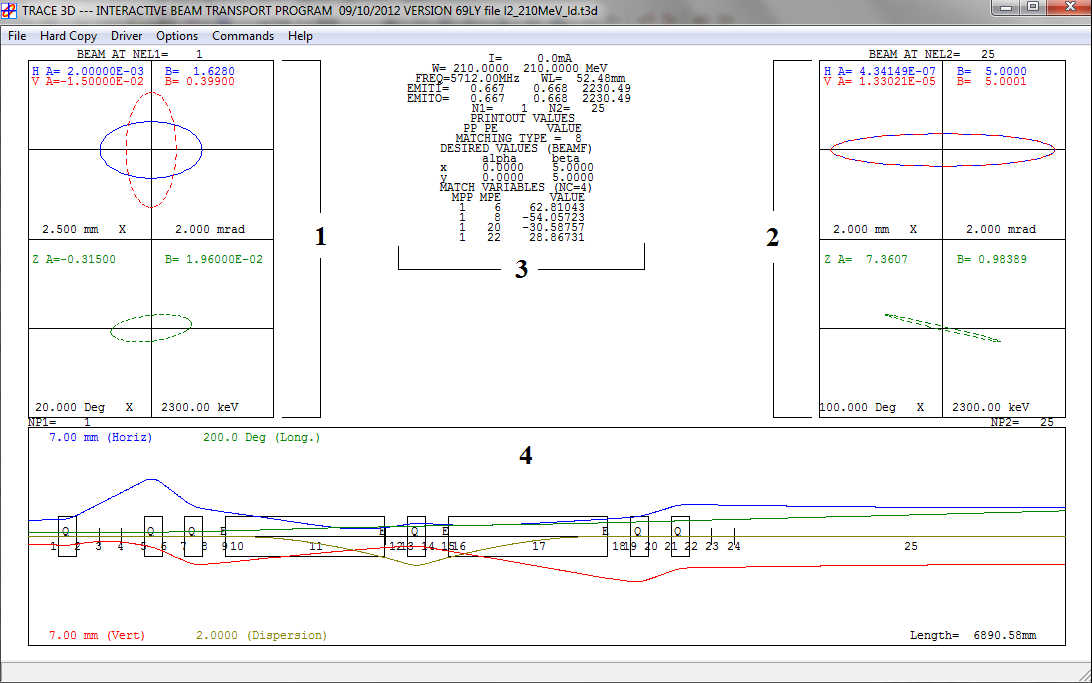
\includegraphics[width=\textwidth-1cm, keepaspectratio=true]{figures/Benchmarks/Trace.png}
    \caption{TRACE 3D graphic interface where: (1) input beam in transverse plane (above) and longitudinal plane (below); (2) output beam in transverse plane (above) and longitudinal plane (below); (3) summary of beam parameters such as input and output emittances and desired value for matching function; (4) line lattice with different elements and beam envelope. The color legend is: blue line for horizontal plane, red line for vertical plane, green line for longitudinal plane and yellow line for dispersion.}
    \label{fig:trace}
\end{figure}
\clearpage
%----------------------------------------------------------------------------------------
%    SECTION 2: TRANSPORT
%----------------------------------------------------------------------------------------
\subsection{TRANSPORT}
\label{sec:TRAN}
TRANSPORT is a computer program for first-order and second-order matrix multiplication, intended for the design of beam transport system \cite{bib:transport}. The TRANSPORT version for Windows provides a graphic beam profile diagram, as well as a sigma matrix description of the simulated beam and line \cite{Transport_GUI}.
Differently from TRACE 3D, the ellipses are characterized by the sigma-matrix coefficients and the Twiss parameters and emittances (total and unnormalized) are reported as output information.
\subsection{TRANSPORT Units}
\label{ssec:TRAN_units}
At any specified position in the system, an arbitrary charged particle is represented by a vector, whose components are positions, angles and momentum of the particle with respect to the reference trajectory. The standard units and internal coordinates in TRANSPORT are:
\begin{itemize}
\item \textbf{horizontal plane:} \\
x [cm] is the displacement of the arbitrary ray with respect to the assumed central trajectory;\\
$\theta$ [mrad] is the angle the ray makes with respect to the assumed central trajectory;
\item \textbf{vertical plane:}\\
y [cm] is the displacement of the arbitrary ray with respect to the assumed central trajectory;\\
$\phi$ [mrad] is the angle the ray makes with respect to the assumed central trajectory;
\item \textbf{longitudinal plane:}\\
l [cm] is the path length difference between the arbitrary ray and the central trajectory;\\
$\delta$ [\%] is the fractional momentum deviation of the ray from the assumed central trajectory.
\end{itemize}
Even if TRANSPORT supports this standard set of units [cm, mrad and \%]; however using \textbf{card 15}, the users can redefine the units (see page 99 on TRANSPORT documentation \cite{bib:transport} for more details).
\subsection{TRANSPORT Input beam}
\label{ssec:TRAN_input}
The input beam is described in \textbf{card 1} in terms of the semi-axes of a six-dimensional erect ellipsoid beam. In terms of diagonal sigma-matrix elements, the input beam in TRANSPORT is expressed by 7 parameters:
\begin{itemize}
\item $\sqrt{\sigma_{ii}}$ [cm] represents one-half of the horizontal (i=1), vertical (i=3) and longitudinal extent (i=5);
\item $\sqrt{\sigma_{ii}}$ [mrad] represents one-half of the horizontal (i=2), vertical (i=4) beam divergence;
\item $\sqrt{\sigma_{66}}$ [\%] represents one-half of the momentum spread;
\item p(0) is the momentum of the central trajectory  [GeV/c].
\end{itemize}
If the input beam is tilted (Twiss alphas not zero), \textbf{ card 12} must be used, inserting the 15 correlations $r_{ij}$ parameters among the 6 beam components. The correlation parameters are defined as following:
\begin{equation}
r_{ij}=\frac{\sigma_{ij}}{\sqrt{\sigma_{ii}\sigma_{jj}}}
\end{equation}
As explained before, with the \textbf{card 15}, it is possible to transform the TRANSPORT standard units in TRACE-like units. In this way, the TRACE 3D sigma-matrix for the input beam, printed out by \textit{command Z}, can be directly used as input beam in TRANSPORT. An example of TRACE 3D sigma-matrix structure is shown in \figref{trace_z}.
\begin{figure}[htbp]
 \centering
     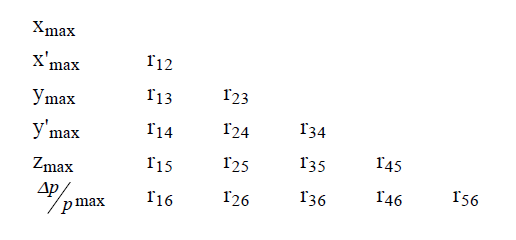
\includegraphics[width=0.5\textwidth-0.6cm, keepaspectratio=true]{figures/Benchmarks/TRACE_z.png}
    \caption{Sigma-matrix structure in TRACE 3D \cite{Trace_man}}
    \label{fig:trace_z}
\end{figure}
From the sigma-matrix coefficients, TRANSPORT reports in output the Twiss parameters and the total, unnormalized emittance. Even in this case, a factor 5 is present between the emittances calculated by TRANSPORT and the corresponding RMS values.
\subsubsection{TRANSPORT Graphic Interface}
\label{ssec:TRAN_graphic}
An improved version of TRANSPORT has been embedded in a new graphic shell written in C++ and is providing GUI type tools, which makes it easier to design new beam lines. A screen shot of a modern GUI Transport interface \cite{Transport_GUI} is shown in \figref{TRANSPORT}.
\begin{figure}[htbp]
 \centering
     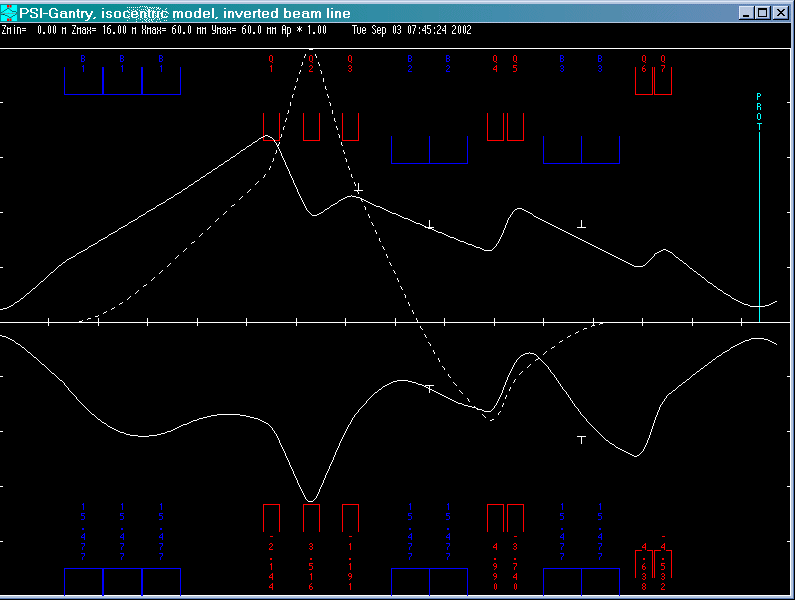
\includegraphics[width=\textwidth-1cm, keepaspectratio=true]{figures/Benchmarks/TRANSPORT.png}
    \caption{GUI TRANSPORT graphic interface \cite{Tran_ex}. The continuous lines describe the beam envelope in the vertical plane (above) and horizontal plane (below). The dashed line displays the dispersion. The elements in the beam line are drawn as blue and red rectangles}
 \label{fig:TRANSPORT}
\end{figure}
%\vspace{4cm}

%----------------------------------------------------------------------------------------
%    SECTION 3: COMPARISON TRACE 3D - TRANSPORT
%----------------------------------------------------------------------------------------
\subsection{Comparison TRACE 3D and TRANSPORT}
\label{sec:T3D_TRAN}
This study has been done following the same trend of the Regression Test in \opal \cite{AMAS}, replacing the electron beam with a same energy proton beam. Due to the different beam rigidity, the bending magnet features have been redefined with a new magnetic field.

The simulated beam transport line contains:
\begin{itemize}
\item drift space (DRIFT 1): 0.250 m length;
\item bending magnet (SBEND or RBEND): 0.250 m radius of curvature;
\item drift space (DRIFT 2): 0.250 m length.
\end{itemize}

Keeping fixed the lattice structure, many similar transport lines have been tested adding entrance and exit edge angles to the bending magnet, changing the bending plane (vertical bending magnet) and direction (right or left). In all the cases, the difficulties arise from the non-achromaticity of the system and an increase in the horizontal and longitudinal emittance is expected. In addition, the coupling between these two planes has to be accurately studied.

In the following paragraph, an example of Sector Bending magnet (SBEND) simulation with entrance and exit edge angles is discussed.

\subsubsection{Input beam}
The starting simulation has been performed with TRACE 3D code. According to \ssecref{T3D_input}, the simulated input beam is described by the following parameters:
\begin{example}
ER = 938.27
W = 7
FREQ = 700
BEAMI = 0.0, 4.0,0.0, 4.0, 0.0, 0.0756
EMITI = 0.730, 0.730, 7.56
\end{example}

Thanks to the TRACE 3D graphic interface, the input beam can immediately be visualized in the three phase plane as shown in \figref{Input_TRACE}.

\begin{figure}[htbp]
 \centering
     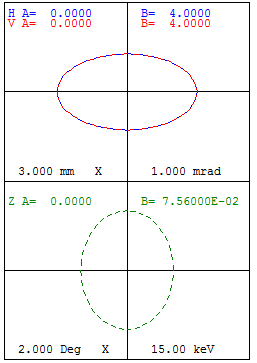
\includegraphics[width=0.5\textwidth-0.6cm, keepaspectratio=true]{figures/Benchmarks/Input_Trace.png}
    \caption{TRACE 3D input beam in the transversal plane (above) and in the longitudinal plane (below)}
    \label{fig:Input_TRACE}
\end{figure}
The corresponding sigma-matrix with the relative units is displayed by command Z:
\begin{figure}[htbp]
 \centering
     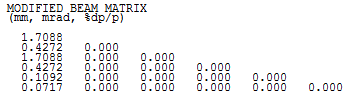
\includegraphics[width=0.5\textwidth-0.6cm, keepaspectratio=true]{figures/Benchmarks/TRACE_z_input.png}
    \caption{TRACE 3D sigma-matrix for the input beam}
    \label{fig:TRACE_z_Input}
\end{figure}
Before entering the TRACE 3D sigma-matrix coefficients in TRANSPORT, a changing in the units is required using the \textbf{card 15} in the following way:
\begin{example}
15. 1. 'MM' 0.1 ; //express in mm the horizontal and vertical beam size
15. 5. 'MM' 0.1 ; //express in mm the beam length
\end{example}

At this point, the TRANSPORT input beam is defined by \textbf{card 1}:
\begin{example}
1.0 1.709 0.427 1.709 0.427 0.11 0.0717 0.1148 /BEAM/ ;
\end{example}

using exactly the same sigma-matrix coefficients of \figref{TRACE_z_Input}. Other two cards must be added in order to use exactly the TRACE 3D R-matrix formalism:
\begin{example}
16. 3. 1863.153; //proton mass, as ratio of electron mass
22. 0.05 0.0 700 0.0 /SPAC/ ; //space charge card
\end{example}
\subsubsection{SBEND in TRACE 3D}
The bending magnet definition in TRACE 3D requires:
\begin{table}[htbp]
\centering
  \caption{Bending magnet description in TRACE 3D and values used in the simulation}
  \label{tab:Bend_Trace}
  \begin{tabular}{|l|l|l|}
  \hline
  \tabhead{Parameter & Value & Description}
  \hline
  NT                  &     8          & Type code for bending \\
  $\alpha$ [deg]      &    30          & angle of bend in horizontal plane \\
  $\rho$ [mm]         &   250          & radius of curvature of central trajectory \\
  n                   &     0          & field-index gradient\\
  vf                  &     0          & flag for vertical bending\\
  \hline
  \end{tabular}
\end{table}
The edge angles are described with another type code and parameters which include also the fringe field. They must be added before and after the bending magnet if entrance and exit edge angles are present and if the fringe field has to be taken into account. In particular for the entrance edge angle:
\begin{table}[htbp]
\centering
  \caption{Edge angle description in TRACE 3D and values used in the simulation}
  \label{tab:Edge_Trace}
  \begin{tabular}{|l|l|l|}
  \hline
  \tabhead{Parameter & Value & Description}
  \hline
  NT                 &     9          & Type code for edge \\
  $\beta$ [deg]      &    10          & pole-face rotation \\
  $\rho$ [mm]        &   250          & radius of curvature of central trajectory \\
  g [mm]             &    20          & total gap of magnet \\
  $K_1$              &   0.36945      & fringe-field factor \\
  $K_2$              &   0.36945      & fringe-field factor \\
  \hline
  \end{tabular}
\end{table}
A same configuration has been used for exit edge angle using $\beta = \SI{5}{\degree}$. The beam envelopes in the three phase planes for this simulation are shown in \figref{Trace_env}.
\begin{figure}[htbp]
 \centering
     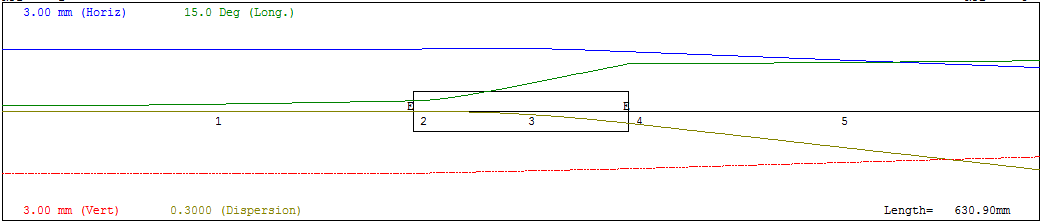
\includegraphics[width=\textwidth-1cm, keepaspectratio=true]{figures/Benchmarks/Trace_SBEND_edge.png}
    \caption{Beam envelopes in TRACE 3D for a SBEND with entrance and exit edge angles. The blue line describes the beam envelope in the horizontal plane, the red line in the vertical plane, the green line in the longitudinal plane. The yellow line displays the dispersion}
    \label{fig:Trace_env}
\end{figure}
\subsubsection{SBEND in TRANSPORT}
The bending magnet definition in TRANSPORT requires:
\begin{table}[htbp]
\centering
\caption{Bending magnet description in TRANSPORT and values used in the simulation}
\label{tab:Bend_Trans}
     \begin{tabular}{|l|l|l|}
        \hline
        \tabhead{Parameter & Value & Description}
        \hline
        Card               & 4     & Type code for bending                      \\
        L [m]              & 30    & Effective length of the central trajectory \\
        $B_0$ [kG]         & 250   & Central field strength                     \\
        n                  & 0     & field-index gradient                       \\
        \hline
       \end{tabular}
\end{table}
As for TRACE 3D, the edge angles are described with another card and parameters. In TRANSPORT, however, the fringe field is not automatically included with the edge angle, but it is described by a own card as reported in the \tabref{Edge_Trans}.
\begin{table}[htbp]
\centering
\caption{Edge angle and fringe field description in TRANSPORT and values used in the simulation}
\label{tab:Edge_Trans}
     \begin{tabular}{|l|l|l|}
        \hline
        \tabhead{Parameter & Value   & Description}
        \hline
        Card               & 2       & Type code for edge         \\
        $\beta$ [deg]      & 10      & pole-face rotation         \\
        \hline
        Card               & 16      & Type code for fringe field \\
        g [mm]             & 10      & half-gap of magnet         \\
        $K_1$              & 0.36945 & fringe-field factor        \\
        $K_2$              & 0.36945 & fringe-field factor        \\
        \hline
        \end{tabular}
\end{table}
Running the Graphic TRANSPORT version, the beam envelopes in the transverse phase planes for this simulation are shown in \figref{Tran_env}.
\begin{figure}[htbp]
 \centering
     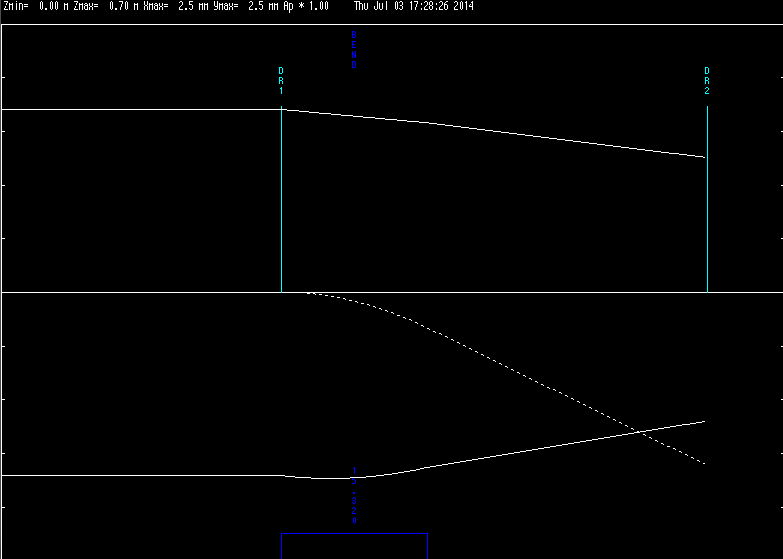
\includegraphics[width=0.5\textwidth-0.6cm, keepaspectratio=true]{figures/Benchmarks/TRANS_SBEND_edge.png}
    \caption{Beam envelopes in TRANSPORT for a SBEND with entrance and exit edge angles. The continuous lines describe the beam envelope in the vertical plane (above) and horizontal plane (below). The dashed line displays the dispersion.}
    \label{fig:Tran_env}
\end{figure}
\subsubsection{Beam size and emittance comparison}
In the next table, the results of the comparison between TRACE 3D and TRANSPORT in terms of the transversal beam sizes at the end of each element in the line are summarized.
\begin{table}[htbp]
\centering
\caption{Transversal beam size at the end of each element in the line printed out by TRACE 3D and TRANSPORT}
\label{tab:Beam_size}
     \begin{tabular}{|l|l|l|l|l|l|}
        \hline
        \multicolumn{2}{|c|}{}    & \multicolumn{2}{c|}{\tabheadcell{TRACE 3D}}  & \multicolumn{2}{c|}{\tabheadcell{TRANSPORT}}     \\
        \hline
        Position    & z (m)       &  $\sigma_x$ (mm)   & $\sigma_y$ (mm)         & $\sigma_x$ (mm)  & $\sigma_y$ (mm)               \\
        %\hline
        Input       & 0.000       &  1.709             &    1.709                &   1.709          & 1.709                         \\
        %\hline
        Drift 1     & 0.250       &  1.712             &    1.712                &   1.712          & 1.712                         \\
        %\hline
        Edge        & 0.250       &  1.712             &    1.712                &   1.712          & 1.712                         \\
        %\hline
        Bend        & 0.381       &  1.638             &    1.587                &   1.638          & 1.587                         \\
        %\hline
        Edge        & 0.381       &  1.638             &    1.587                &   1.638          & 1.587                         \\
        %\hline
        Drift 2     & 0.631       &  1.206             &    1.264                &   1.206          & 1.264                         \\
        \hline
        \end{tabular}
\end{table}
The perfect agreement between these two codes arises immediately looking at \figref{T3D_Tra_env}.
\begin{figure}[htbp]
 \centering
     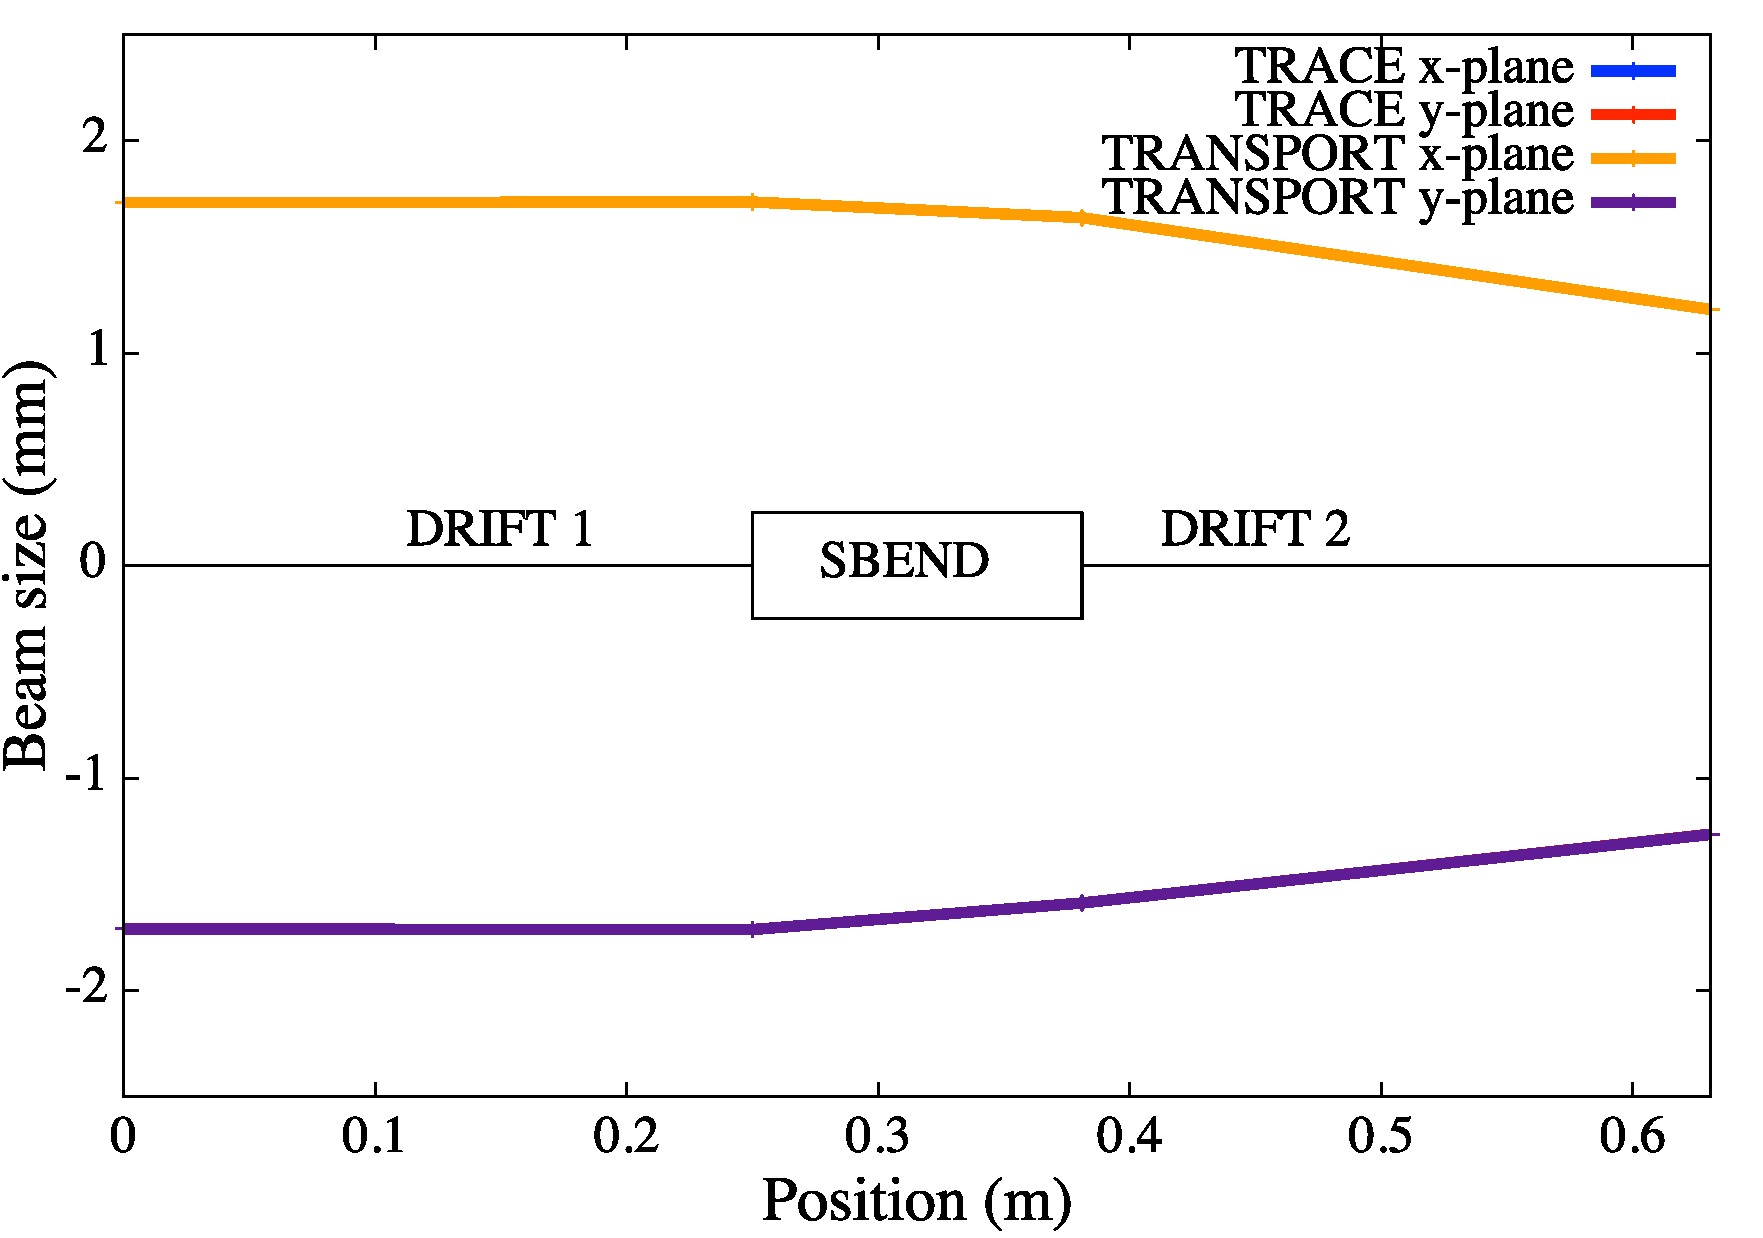
\includegraphics[width=0.5\textwidth-1cm, keepaspectratio=true]{figures/Benchmarks/T3D_Tra_SBEND_edge_env.pdf}
    \caption{Transversal beam size comparison between TRACE 3D and TRANSPORT}
    \label{fig:T3D_Tra_env}
\end{figure}
The same comparison has been performed in terms of horizontal and longitudinal emittance, both expressed in $\pi$-mm-mrad. While the vertical emittance remains constant and equal to the initial value ($\epsilon_y = $ 0.730 $\pi$-mm-mrad) , the horizontal and longitudinal emittances are expected growing after the bending magnet. The results are reported in \tabref{Emittance} and in \figref{T3D_Tra_emi}.
\begin{table}[htbp]
\centering
\caption{Horizontal and longitudinal emittance comparison between TRACE 3D and TRANSPORT, both expressed in $\pi$-mm-mrad}
\label{tab:Emittance}
     \begin{tabular}{|l|l|l|l|l|l|}
        \hline
        \multicolumn{2}{|c|}{}       & \multicolumn{2}{c|}{\tabheadcell{TRACE 3D}}     & \multicolumn{2}{c|}{\tabheadcell{TRANSPORT}}\\
        \hline
        Position     & z (m)         &  $\epsilon_x$   &   $\epsilon_z$               &   $\epsilon_x$   & $\epsilon_z$              \\
        %\hline
        Input        &     0         &  0.730          &    0.08                      &   0.730          & 0.08                      \\
        %\hline
        Drift 1      &     0.250     &  0.730          &    0.08                      &   0.730          & 0.08                      \\
        %\hline
        Edge         &     0.250     &  0.730          &    0.08                      &   0.730          & 0.08                      \\
        %\hline
        Bend         &     0.381     &  0.973          &    0.65                      &   0.973          & 0.65                      \\
        %\hline
        Edge         &     0.381     &  0.973          &    0.65                      &   0.973          & 0.65                      \\
        %\hline
        Drift 2      &     0.631     &  0.973          &    0.65                      &   0.973          & 0.65                      \\
        \hline
        \end{tabular}
\end{table}
\begin{figure}[htbp]
 \centering
     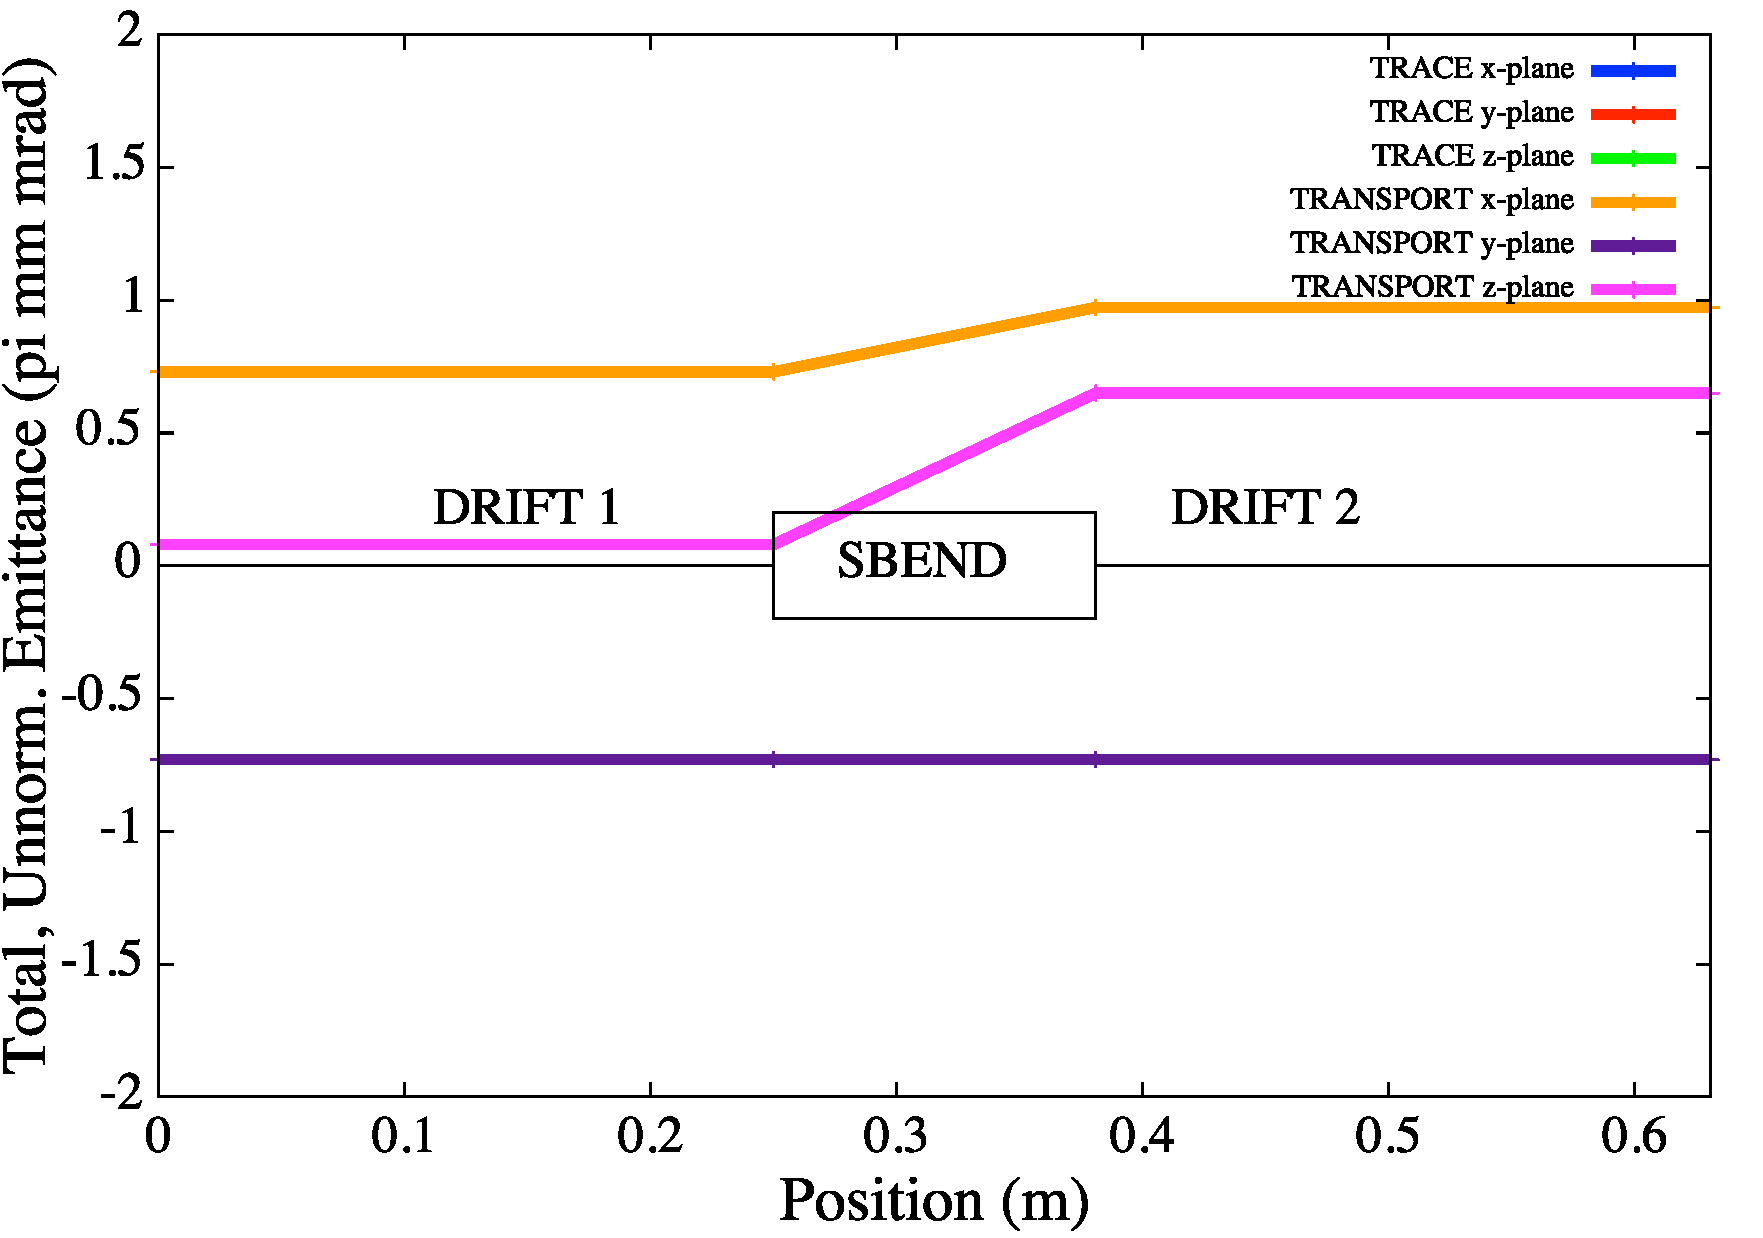
\includegraphics[width=0.5\textwidth-1cm, keepaspectratio=true]{figures/Benchmarks/T3D_Tra_SBEND_edge_emi.pdf}
    \caption{Emittance comparison between TRACE and TRANSPORT}
    \label{fig:T3D_Tra_emi}
\end{figure}

\subsubsection{From TRACE 3D to TRANSPORT}
\label{ssec:T3DtoTRAN}

\begin{table}[!ht]
\centering
\caption{Bending magnet features in TRACE 3D and TRANSPORT}
\label{tab:Bend_Trace_Tra2}
     \begin{tabular}{|l|l|l|}
        \hline
        \tabhead{Parameter         & Trace 3D              & Transport}
        \hline
        \textbf{Bend card}         & 8                     & 4                        \\
        Angle                      & Input parameter [deg] & Output information [deg] \\
        Magn. field                & Calculated. [T]       & Input parameter [kG]     \\
        Radius of curv.            & Input parameter [mm]  & Output information [m]   \\
        Field-index                & Input parameter       & Input parameter          \\
        Effect. length             & Calculated [mm]       & Input parameter [m]      \\
        \hline
        \hline
        \textbf{Edge card}         & 9                     & 2                        \\
        Edge angle                 & Input parameter [deg] & Input parameter [deg]    \\
        \hline
        \hline
        \textbf{Vertical gap}      & 9                     & 16.5                     \\
        Gap                        & Total [mm]            & Half-gap [cm]            \\
        \hline
        \hline
        \textbf{Fringe field card} & 9                     & 16.7 / 16.8              \\
        $K_1$                      & Default: 0.45         & Default: 0.5             \\
        $K_2$                      & Default: 2.8          & Default: 0               \\
        \hline
        \hline
        \textbf{Bend direction}    & Bend angle sign       & Coord. rotation          \\
        Horiz. right               & Angle $>$ 0           & Angle $>$ 0              \\
        Horiz. left                & Angle $<$ 0           & Card 20                  \\
        Vertical bend              & Card 8, vf $>$ 0      & Card 20                  \\
        \hline
        \end{tabular}
\end{table}

\clearpage
%----------------------------------------------------------------------------------------
%    SECTION: \opal
%----------------------------------------------------------------------------------------

\subsection{Relations to \opalt}
\label{sec:OPAL}

In \opal, the beam dynamics approach (time integration) is hence completely different from the envelope-like supported by TRACE 3D and TRANSPORT. The three codes support different units and require diverse parameters for the input beam. A summary of their main features is reported in \tabref{Features}.

\begin{table}[htbp]
    \centering
\caption{Main features of the three beam dynamics codes: TRACE 3D, TRANSPORT and \opal}
\label{tab:Features}
        \begin{tabular}{|l|l|l|l|}
        \hline
        \tabhead{Code  & TRACE 3D          & TRANSPORT          & \opal}
        \hline
        \textbf{Type}  & Envelope          & Envelope           & Time integration \\
        %\hline
        \textbf{Input} & Twiss, Emittance  & Sigma, Momentum    & Sigma, Energy    \\
        %\hline
        \textbf{Units} & mm-mrad, deg-keV  & cm-rad, cm-\%      & m-$\beta\gamma$  \\
        \hline
\end{tabular}
\end{table}

\subsection{\opalt Units}
\label{ssec:OPAL_units}

\opalt supports the following internal coordinates and units for the three phase planes:

\begin{itemize}
\item \textbf{horizontal plane:} \\
X [m] horizontal position of a particle relative to the axis of the element;\\
PX [$\beta_x\gamma$] horizontal canonical momentum;

\item \textbf{vertical plane:}\\
Y [m] vertical position of a particle relative to the axis of the element;\\
PY [$\beta_y\gamma$] horizontal canonical momentum;

\item \textbf{longitudinal plane:}\\
Z [m] longitudinal position of a particle in floor-coordinates;\\
PZ [$\beta_z\gamma$] longitudinal canonical momentum;
\end{itemize}

\subsection{\opalt Input beam}
\label{ssec:OPAL_input}

For the input beam, a \texttt{GAUSS} distribution type has been chosen.  For transferring the TRANSPORT (or TRACE 3D) input beam in terms of sigma-matrix coefficients, it necessary to:

\begin{itemize}
\item  adjust the units: from mm to m;
\item correct for the factor $\sqrt{5}$: from total to RMS distribution;
\item multiply for the relativistic factor $\beta\gamma =\num{0.1224}$ for \SI{7}{\mega\electronvolt} protons;
\end{itemize}

 In case of the modified sigma-matrix in \figref{TRACE_z_Input}, the corresponding \opal parameters for the \texttt{GAUSS} distributions are:

\begin{example}
 T3D SIGMA                        OPAL -T
-------------------------------------------------------
1.7088 mm             SIGMAX  = 1.7088/sqrt(5)e-3         m
0.4272 mrad           SIGMAPX = 0.4272/sqrt(5)*0.1224e-3
1.7088 mm             SIGMAY  = 1.7088/sqrt(5)e-3        m
0.4272 mrad           SIGMAPY = 0.4272/sqrt(5)*0.1224e-3
0.1092 mm             SIGMAZ  = 0.1092/sqrt(5)e-3        m
0.0717 %              SIGMAPZ = (0.0717*10)/sqrt(5)*0.1224e-3
\end{example}

At the end of this calculation, the input beam in \opal is:

\begin{example}
D1: DISTRIBUTION, DISTRIBUTION=GAUSS,
SIGMAX = 0.7642e-03,  SIGMAPX= 0.0234e-03,  CORRX= 0.0,
SIGMAY = 0.7642e-03,  SIGMAPY= 0.0234e-03,  CORRY= 0.0,
SIGMAZ = 0.0488e-03,  SIGMAPZ= 0.0392e-03,  CORRZ= 0.0, R61= 0.0,
INPUTMOUNITS=NONE;
\end{example}

%----------------------------------------------------------------------------------------
%    SECTION: Comparison TRACE 3D and OPAL
%----------------------------------------------------------------------------------------

\subsection{Comparison TRACE 3D and \opalt}
\label{sec:T3D_OPAL}

In this section, the comparison between TRACE 3D and \opalt is discussed starting from \keyword{SBEND} definition in \opalt. The transport line described in \secref{T3D_TRAN} has been simulated in \opal using 10.000 particles and $10^{-11}$ s time step. The bending magnet features of \tabref{Bend_Trace,Edge_Trace} have been transformed in \opal language as:

\begin{example}
Bend: SBEND, ANGLE = 30.0 * Pi/180.0,
             K1=0.0,
             E1=0, E2=0,
             FMAPFN = "1DPROFILE1-DEFAULT",
             ELEMEDGE = 0.250,  // end of first drift
             DESIGNENERGY = 7E+06,  // ref energy eV
             L = 0.1294,
             GAP = 0.02;
\end{example}

\begin{itemize}

\item \textbf{SBEND without edge angles:}

\begin{example}
// Bending magnet configuration:
K1=0.0,
E1=0, E2=0,
\end{example}

\begin{figure}[htbp]
\begin{center}
    \subfloat[Transverse beam size]{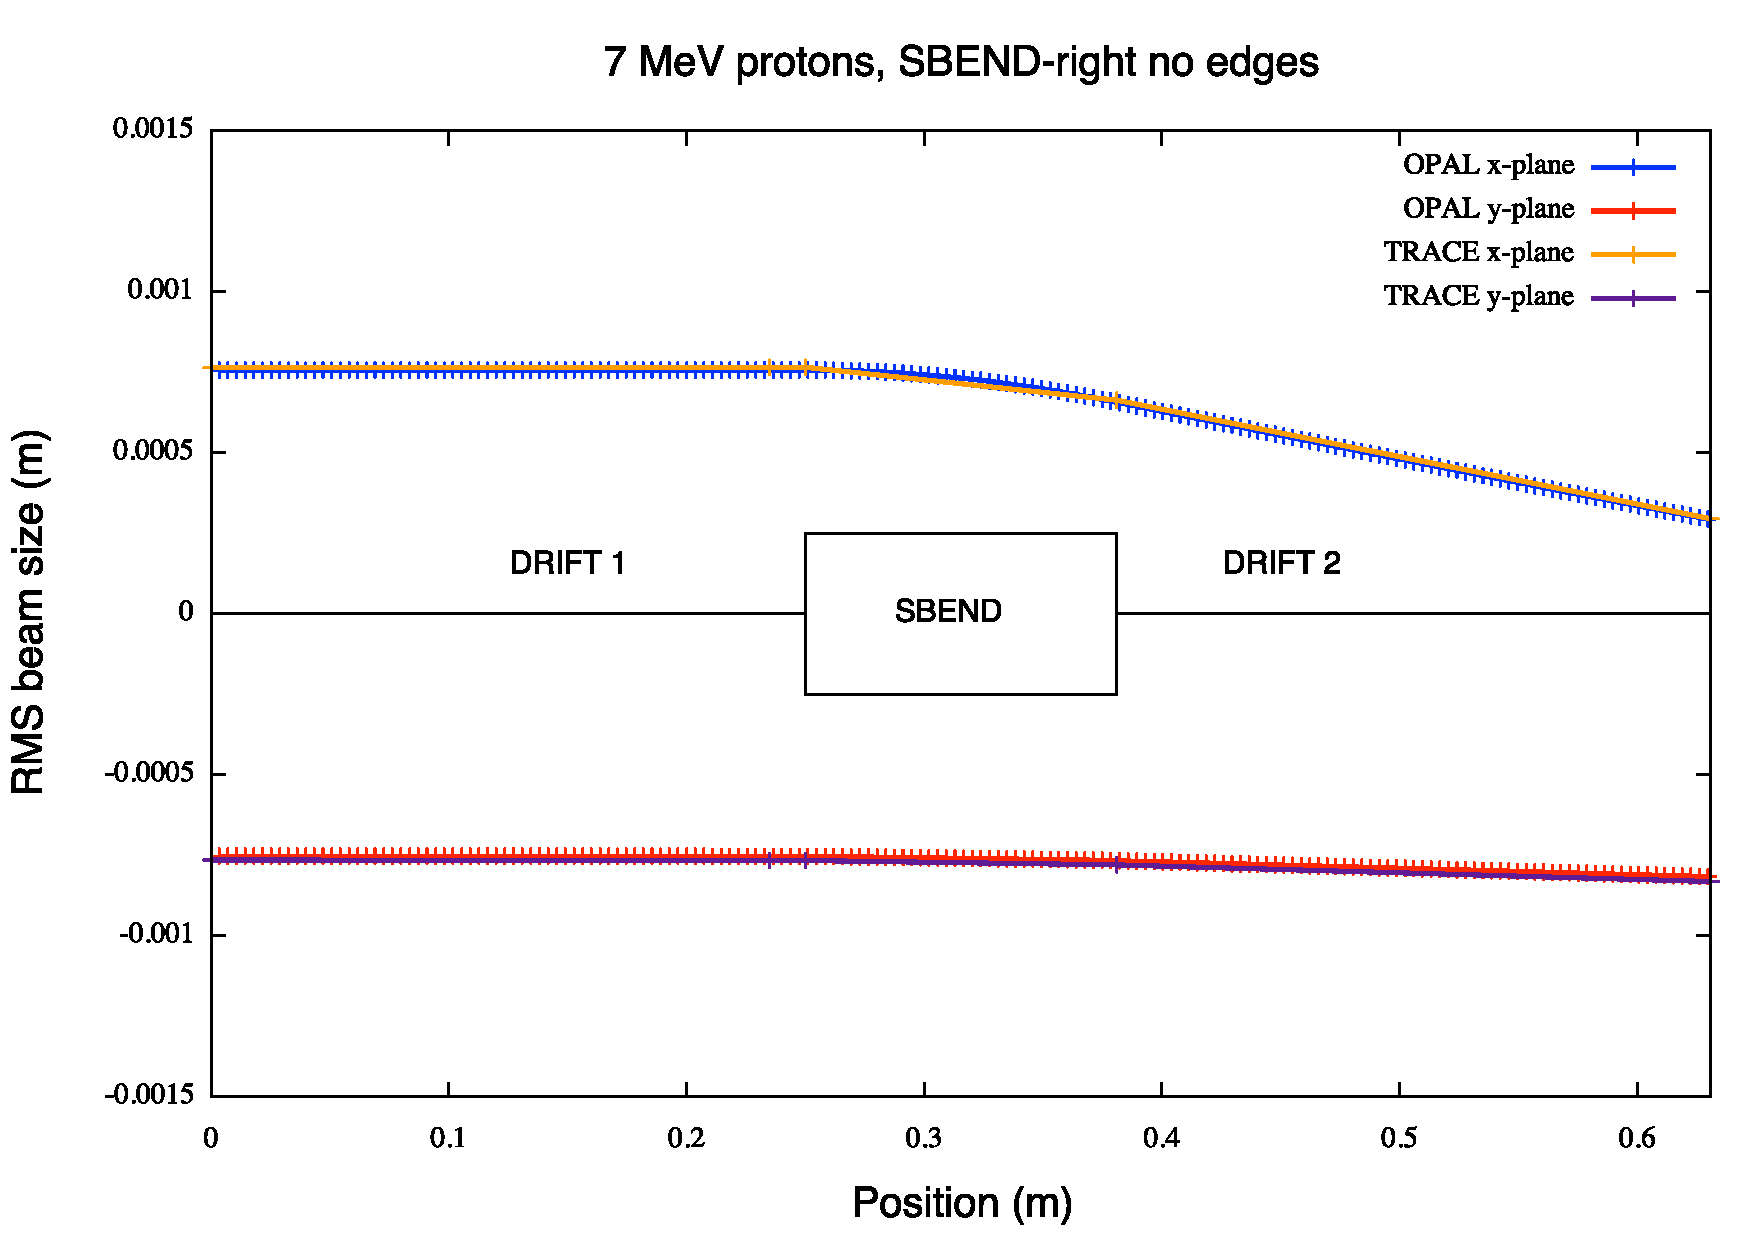
\includegraphics[width=0.5\textwidth-1cm, keepaspectratio=true]{figures/Benchmarks/SBEND_noEdge_Env}}
    \hspace{1.8cm}
    \subfloat[Transverse emittance]{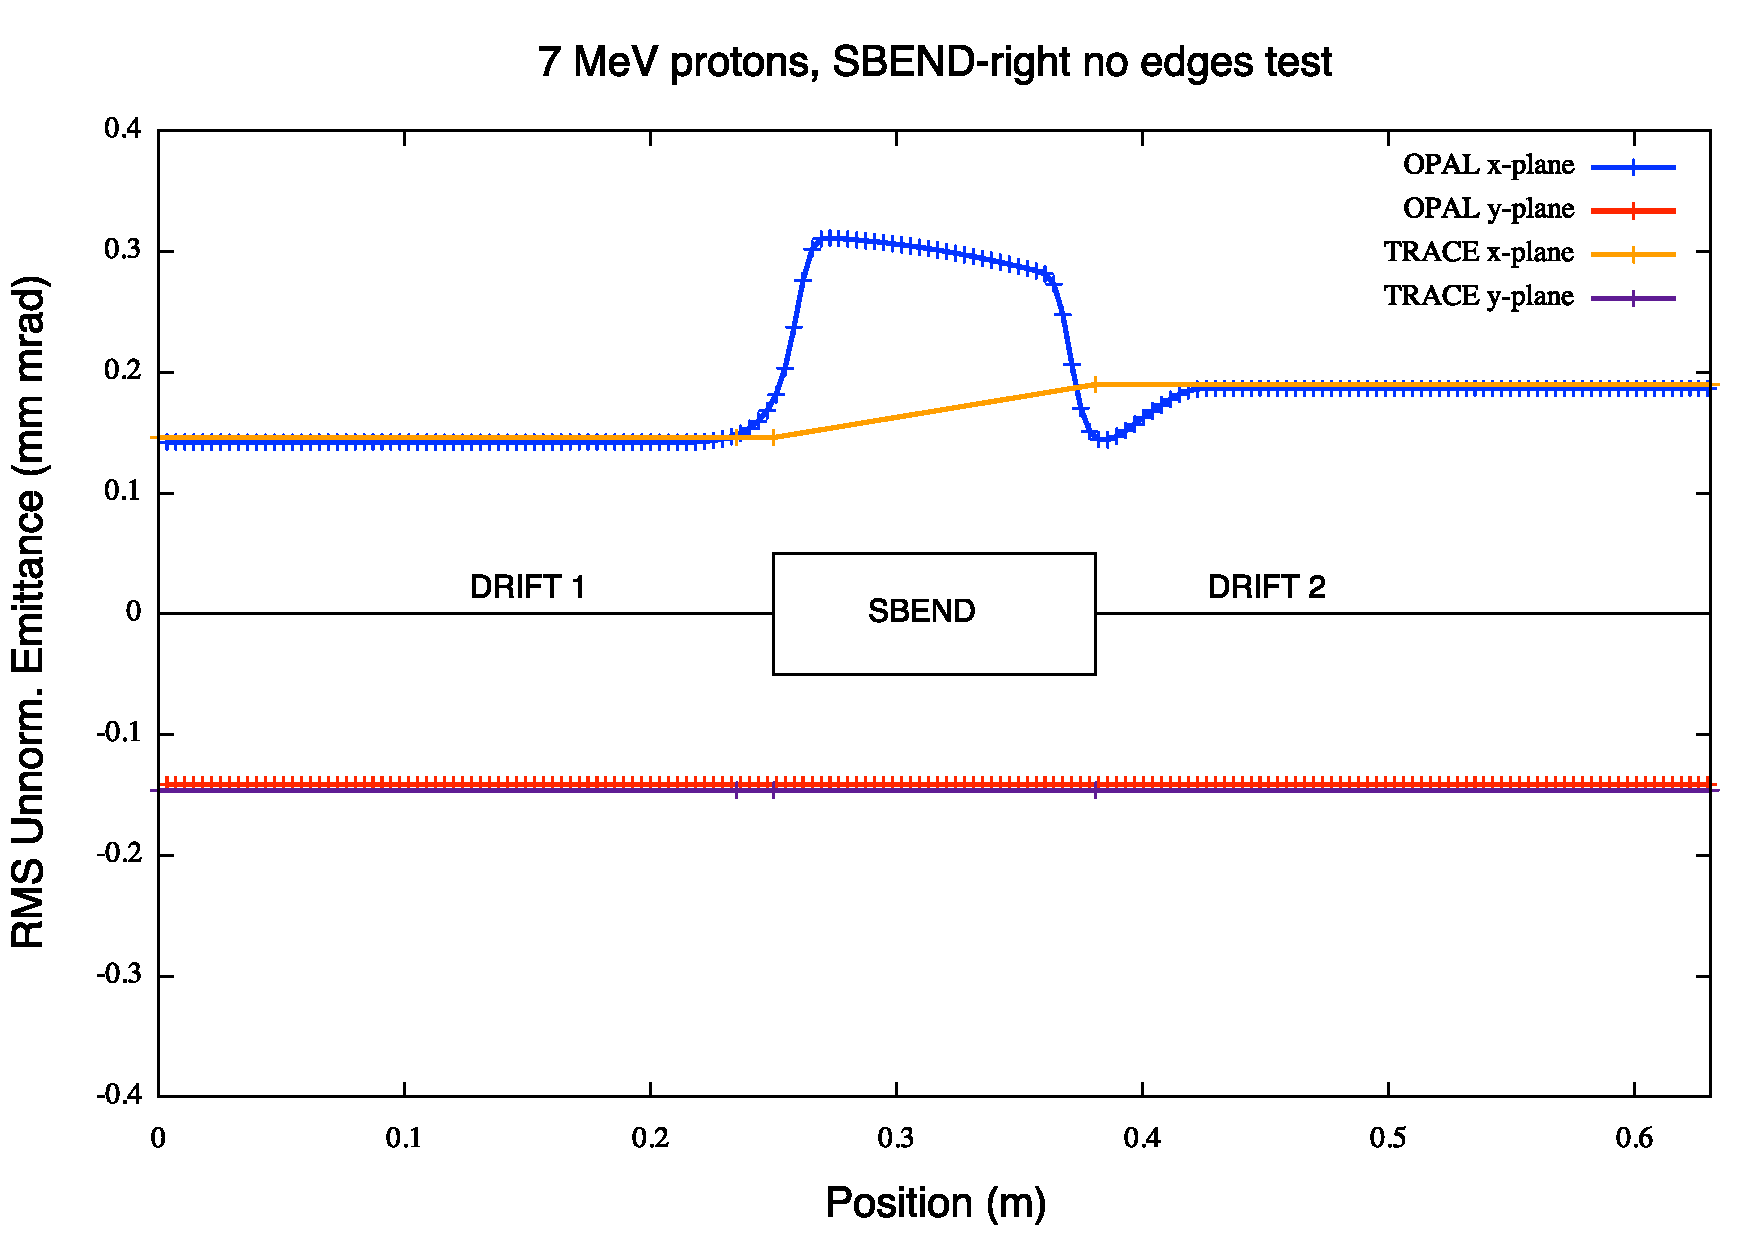
\includegraphics[width=0.5\textwidth-1cm, keepaspectratio=true]{figures/Benchmarks/SBEND_noEdge_Emi}}
    \caption{TRACE 13D and \opal comparison: SBEND without edge angles}
    \label{fig:SBEND_noEdge}
\end{center}
 \end{figure}

A good overall agreement has been found between the two codes in term of beam size and emittance. The different behavior inside the bending magnet for the horizontal emittance is still undergoing study and it's probably due to a diverse coordinate system in the two codes.

\item \textbf{SBEND with edge angles:}

\begin{example}
// Bending magnet configuration:
K1=0.0,
E1=10*Pi/180.0, E2=5* Pi/180.0,
\end{example}


\begin{figure}[htbp]
\begin{center}
    \subfloat[Transverse beam size]{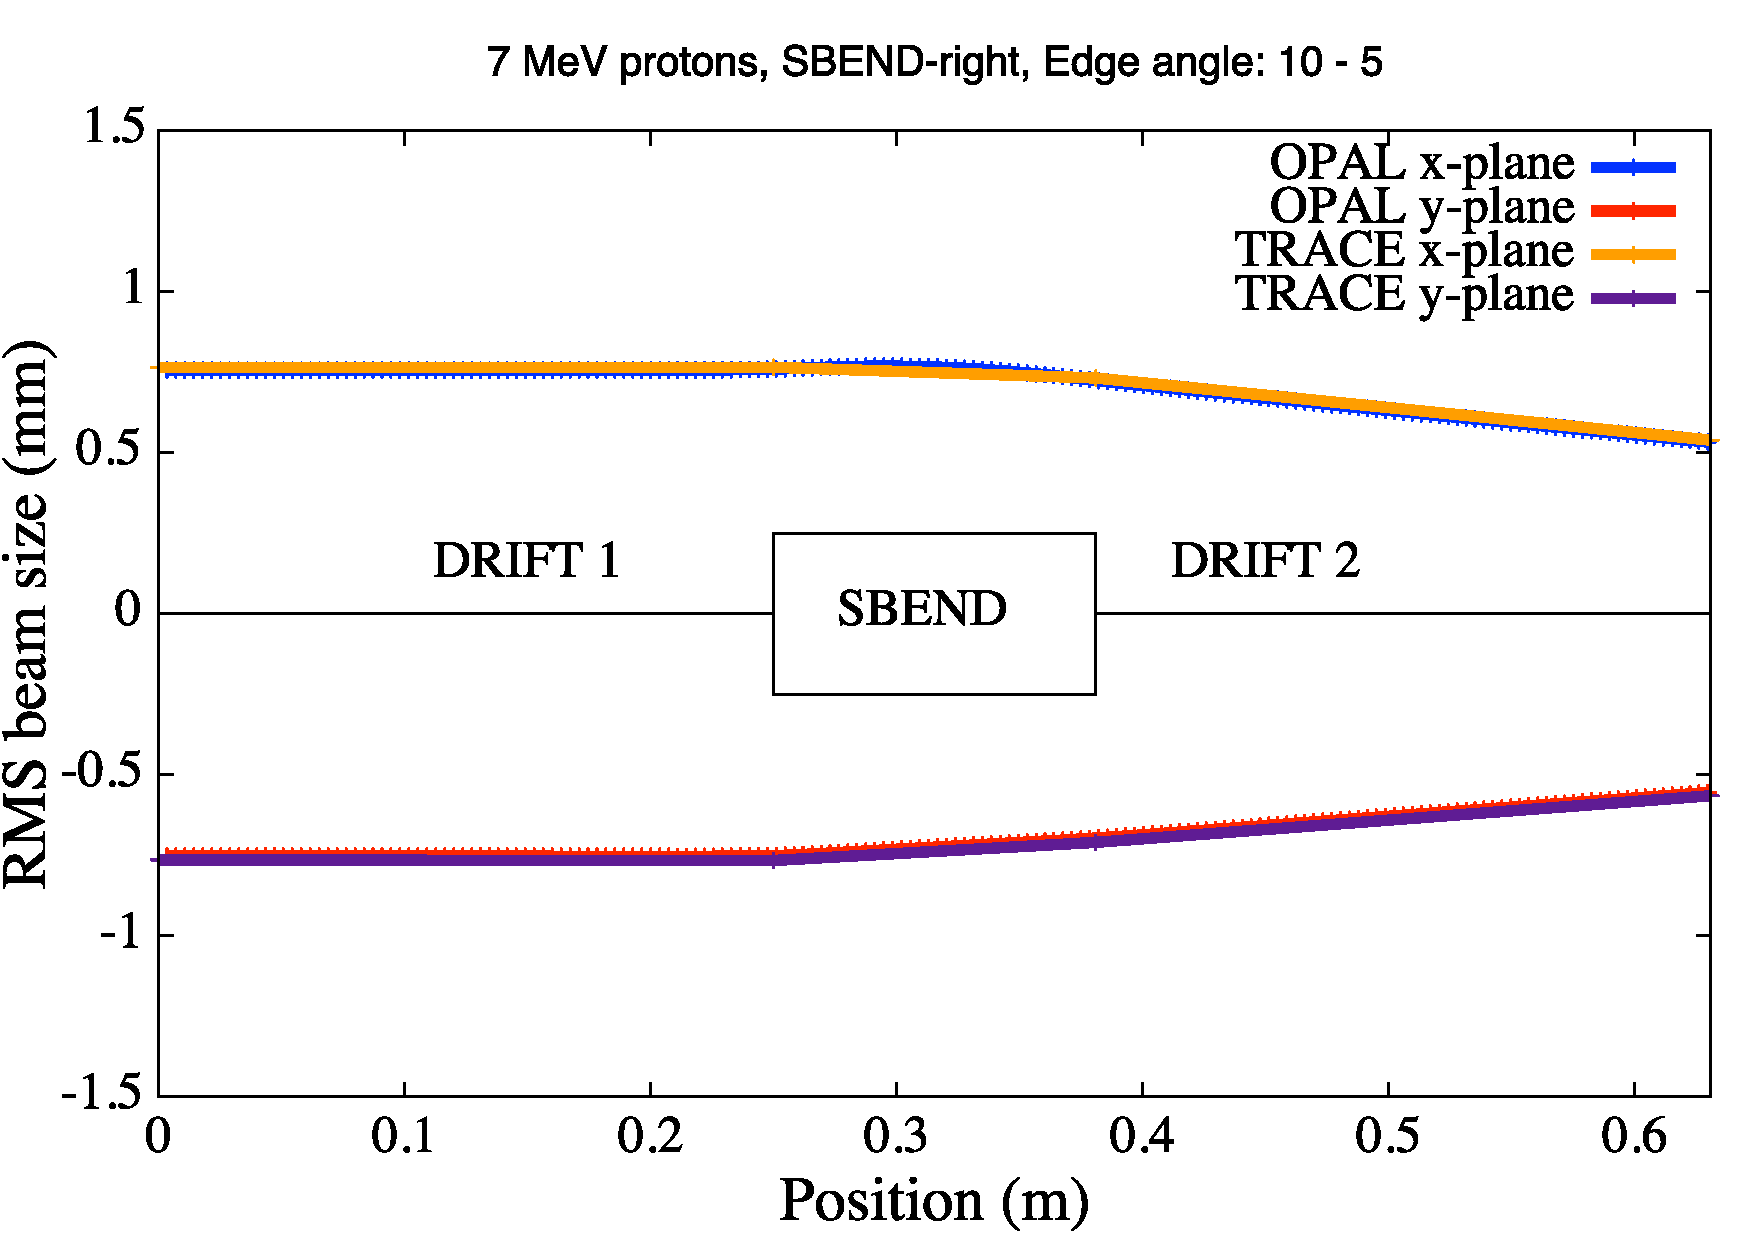
\includegraphics[width=0.5\textwidth-1cm, keepaspectratio=true]{figures/Benchmarks/SBEND_Edges_Env.pdf}}
    \hspace{1.8cm}
    \subfloat[Transverse RMS emittance]{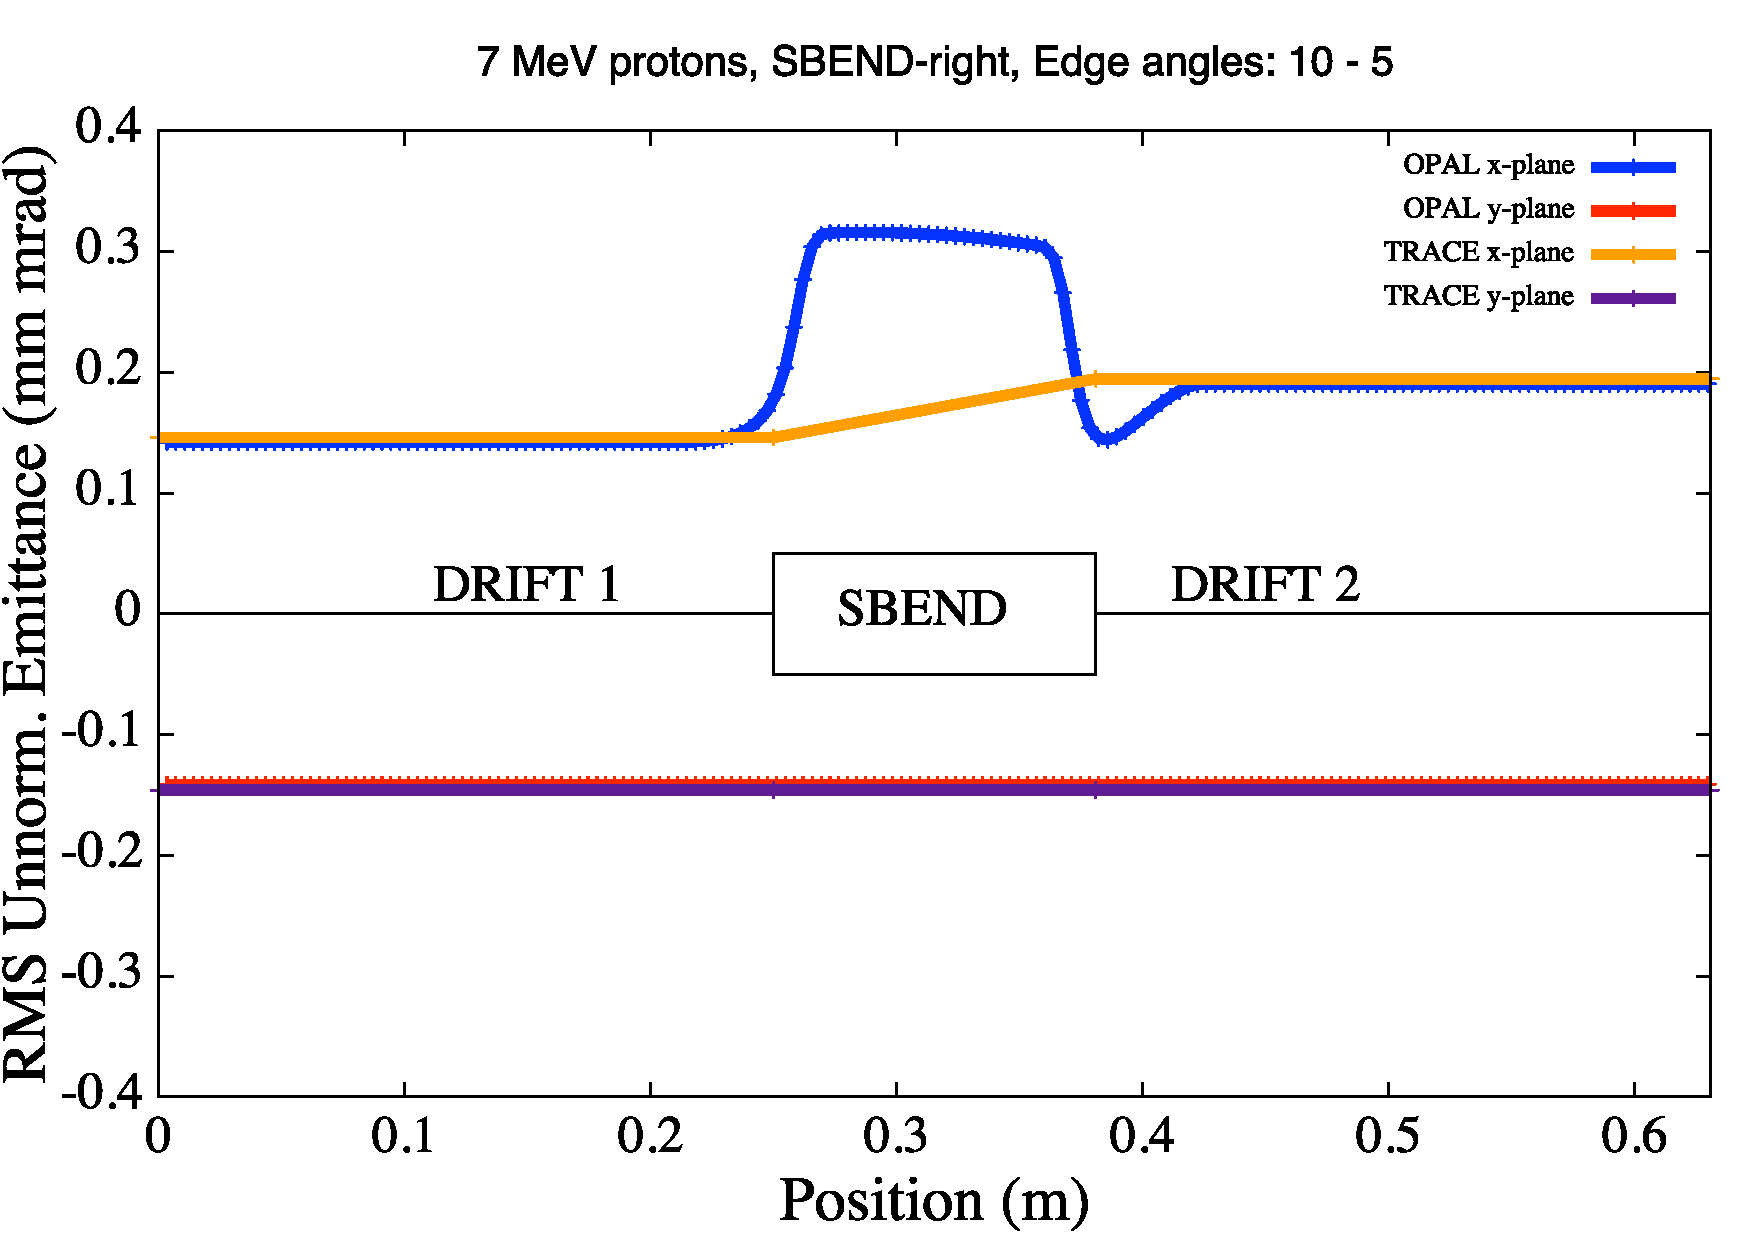
\includegraphics[width=0.5\textwidth-1cm, keepaspectratio=true]{figures/Benchmarks/SBEND_Edges_Emi.pdf}}
    \caption{TRACE 3D and \opal comparison: SBEND with edge angles}
    \label{fig:SBEND_Edges}
\end{center}
 \end{figure}

Even in this case, a good overall agreement has been found between the two codes in term of beam size and emittance.

\item \textbf{SBEND with field index:}

The field index parameter K1 is defined as:

\begin{equation}
K1 = \frac{1}{B\rho}\diffp{B_y}{x},
\end{equation}

\ssecref{RBend}. Instead, in TRACE 3D the field index parameter n is:

\begin{equation}
n = -\frac{\rho}{B_y}\diffp{B_y}{x}.
\end{equation}

In order to have a significant focusing effect on both transverse planes, the transport line has been simulated in TRACE 3D using $n = 1.5$. Since, a different definition exists between \opal and TRACE 3D on the field index, the n-parameter translation in \opal language has been done with the following tests:

\begin{itemize}[noitemsep]
\item[] TEST 1: K1 $=$ n/$\rho^2$
\item[] TEST 2: K1 $=$ n
\item[] TEST 3: K1 $=$ n/$\rho$
\end{itemize}

Only the TEST 2 reports a reasonable behavior on the beam size and emittance, as shown in \figref{SBEND_FI} using:

\begin{example}
// Bending magnet configuration:
K1=1.5
E1=0, E2=0,
\end{example}

\begin{figure}[htbp]
\begin{center}
    \subfloat[Transverse beam size]{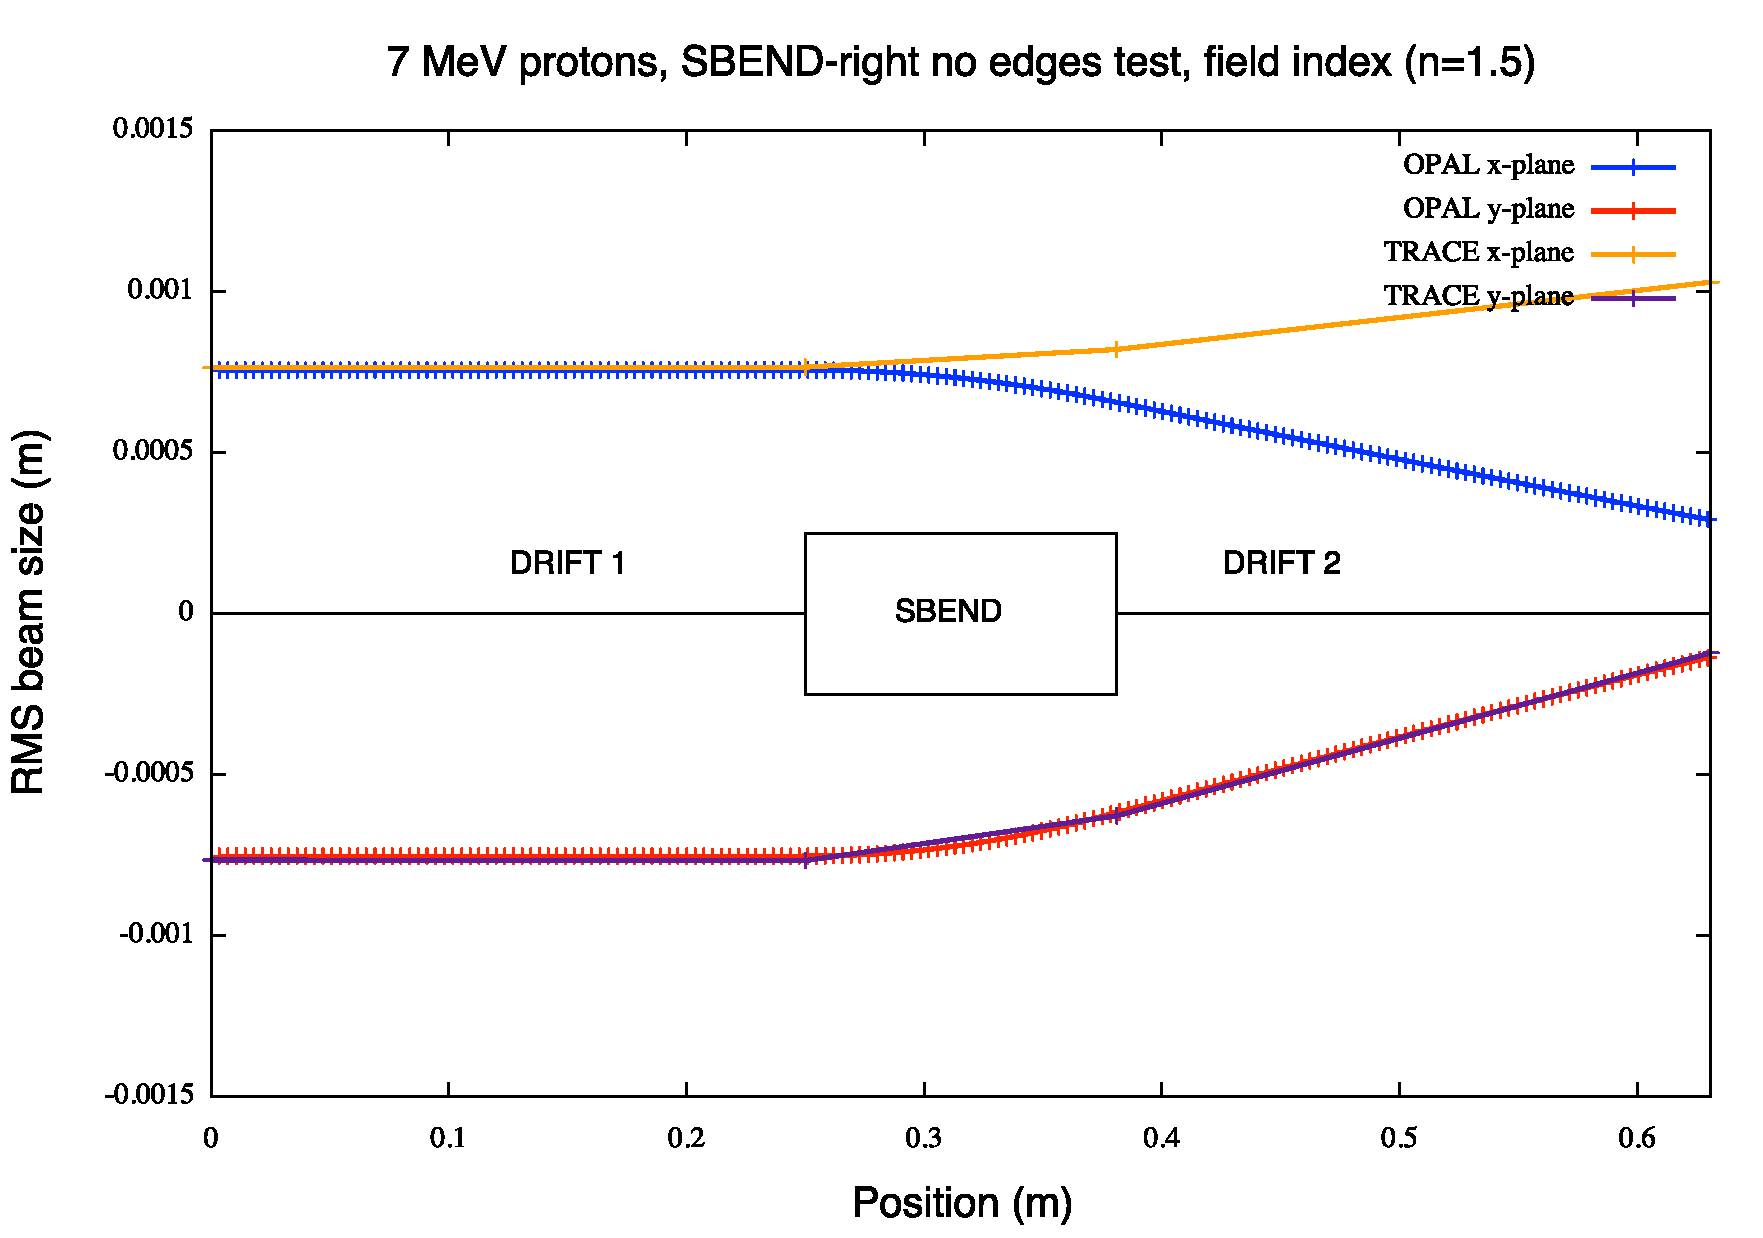
\includegraphics[width=0.5\textwidth-1cm, keepaspectratio=true]{figures/Benchmarks/FI_SBEND_FMDef_Env_T2.pdf}}
    \hspace{1.8cm}
    \subfloat[Transverse RMS emittance]{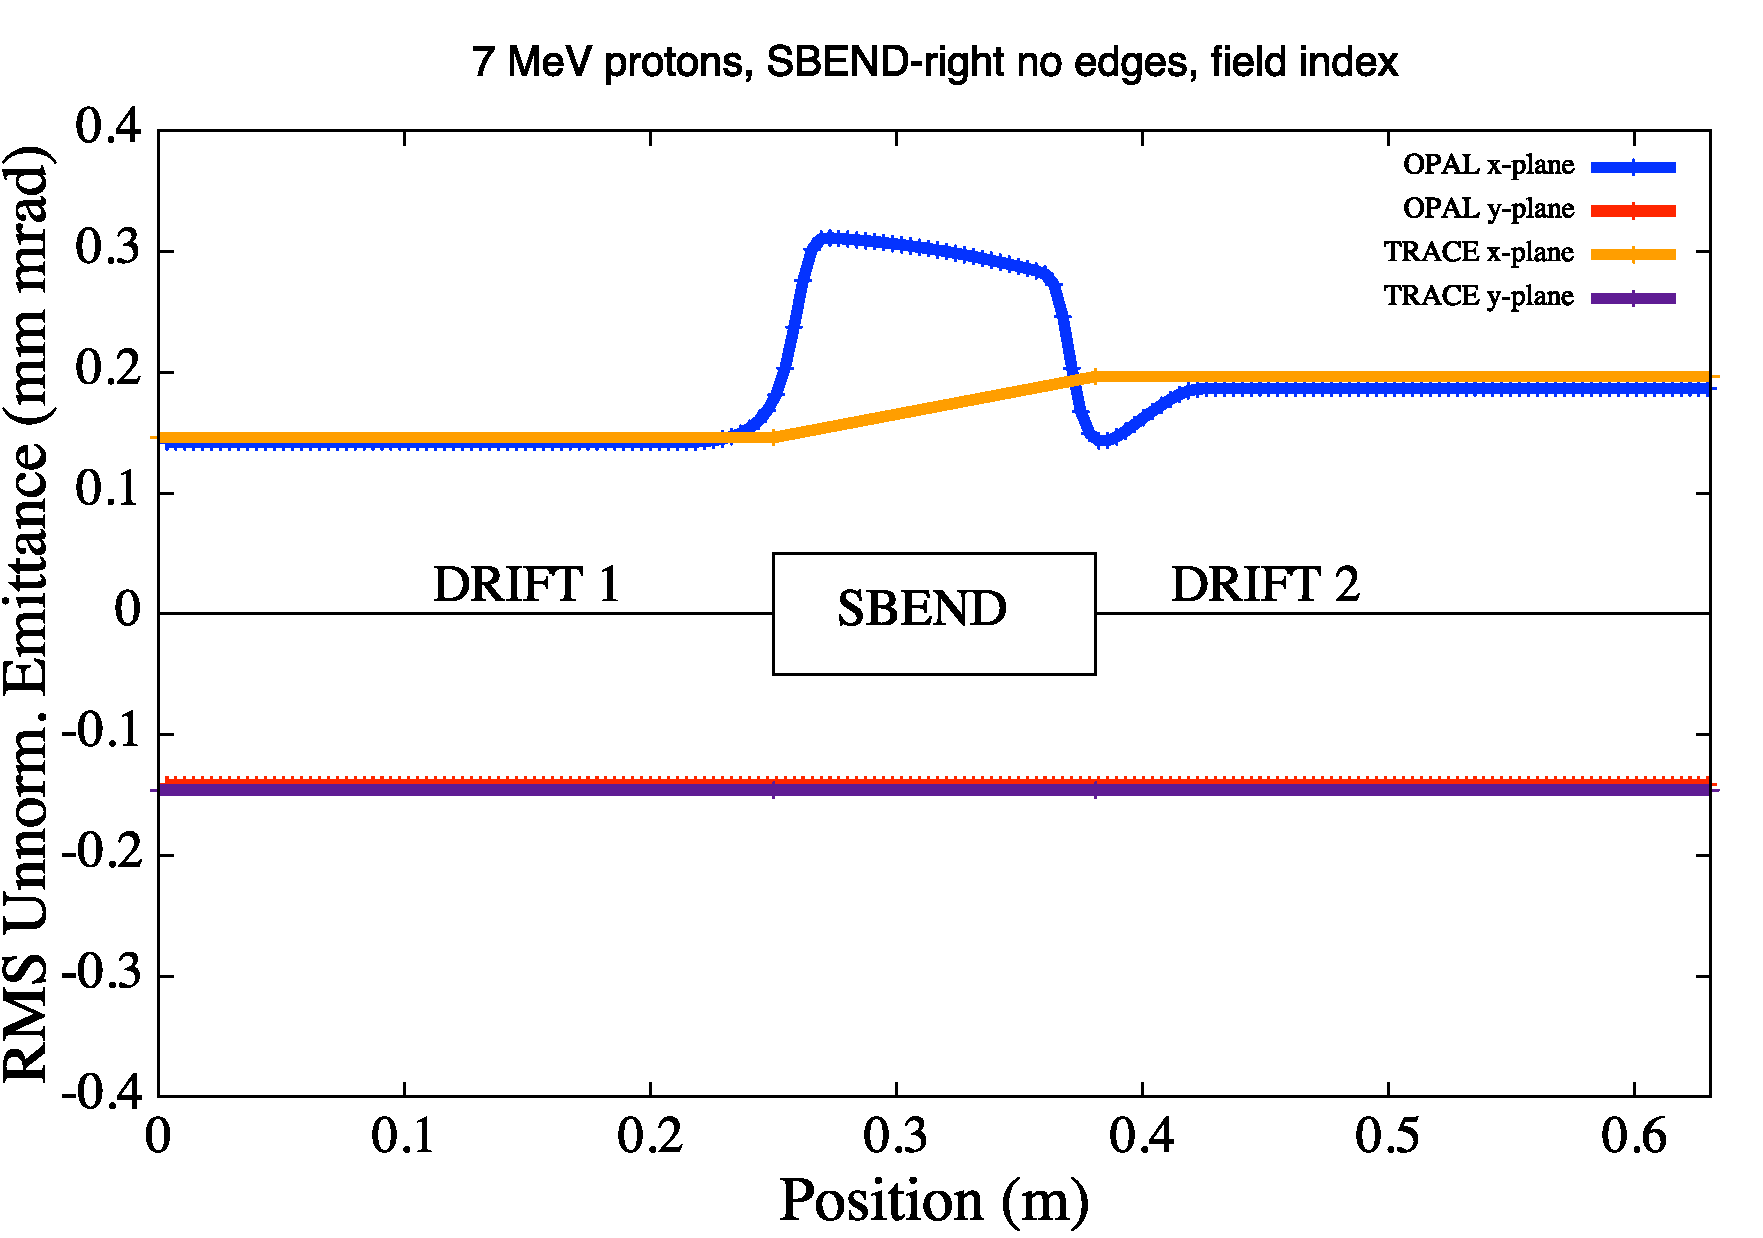
\includegraphics[width=0.5\textwidth-1cm, keepaspectratio=true]{figures/Benchmarks/FI_SBEND_FMDef_Emi_T2.pdf}}
    \caption{TRACE 3D and \opal comparison: SBEND with field index and default field map}
    \label{fig:SBEND_FI}
\end{center}
 \end{figure}

Concerning the emittances and vertical beam size, a perfect agreement has been found, instead a defocusing effect appears in the horizontal plane. These results have been obtained with the default field map provided by \opal. However, a better result, only in the beam size as shown in \figref{SBEND_FI_test}, is achieved using a test field map in which the fringe field extension has been changed in the thin lens approximation.

\begin{figure}[htbp]
\begin{center}
    \subfloat[Transverse beam size]{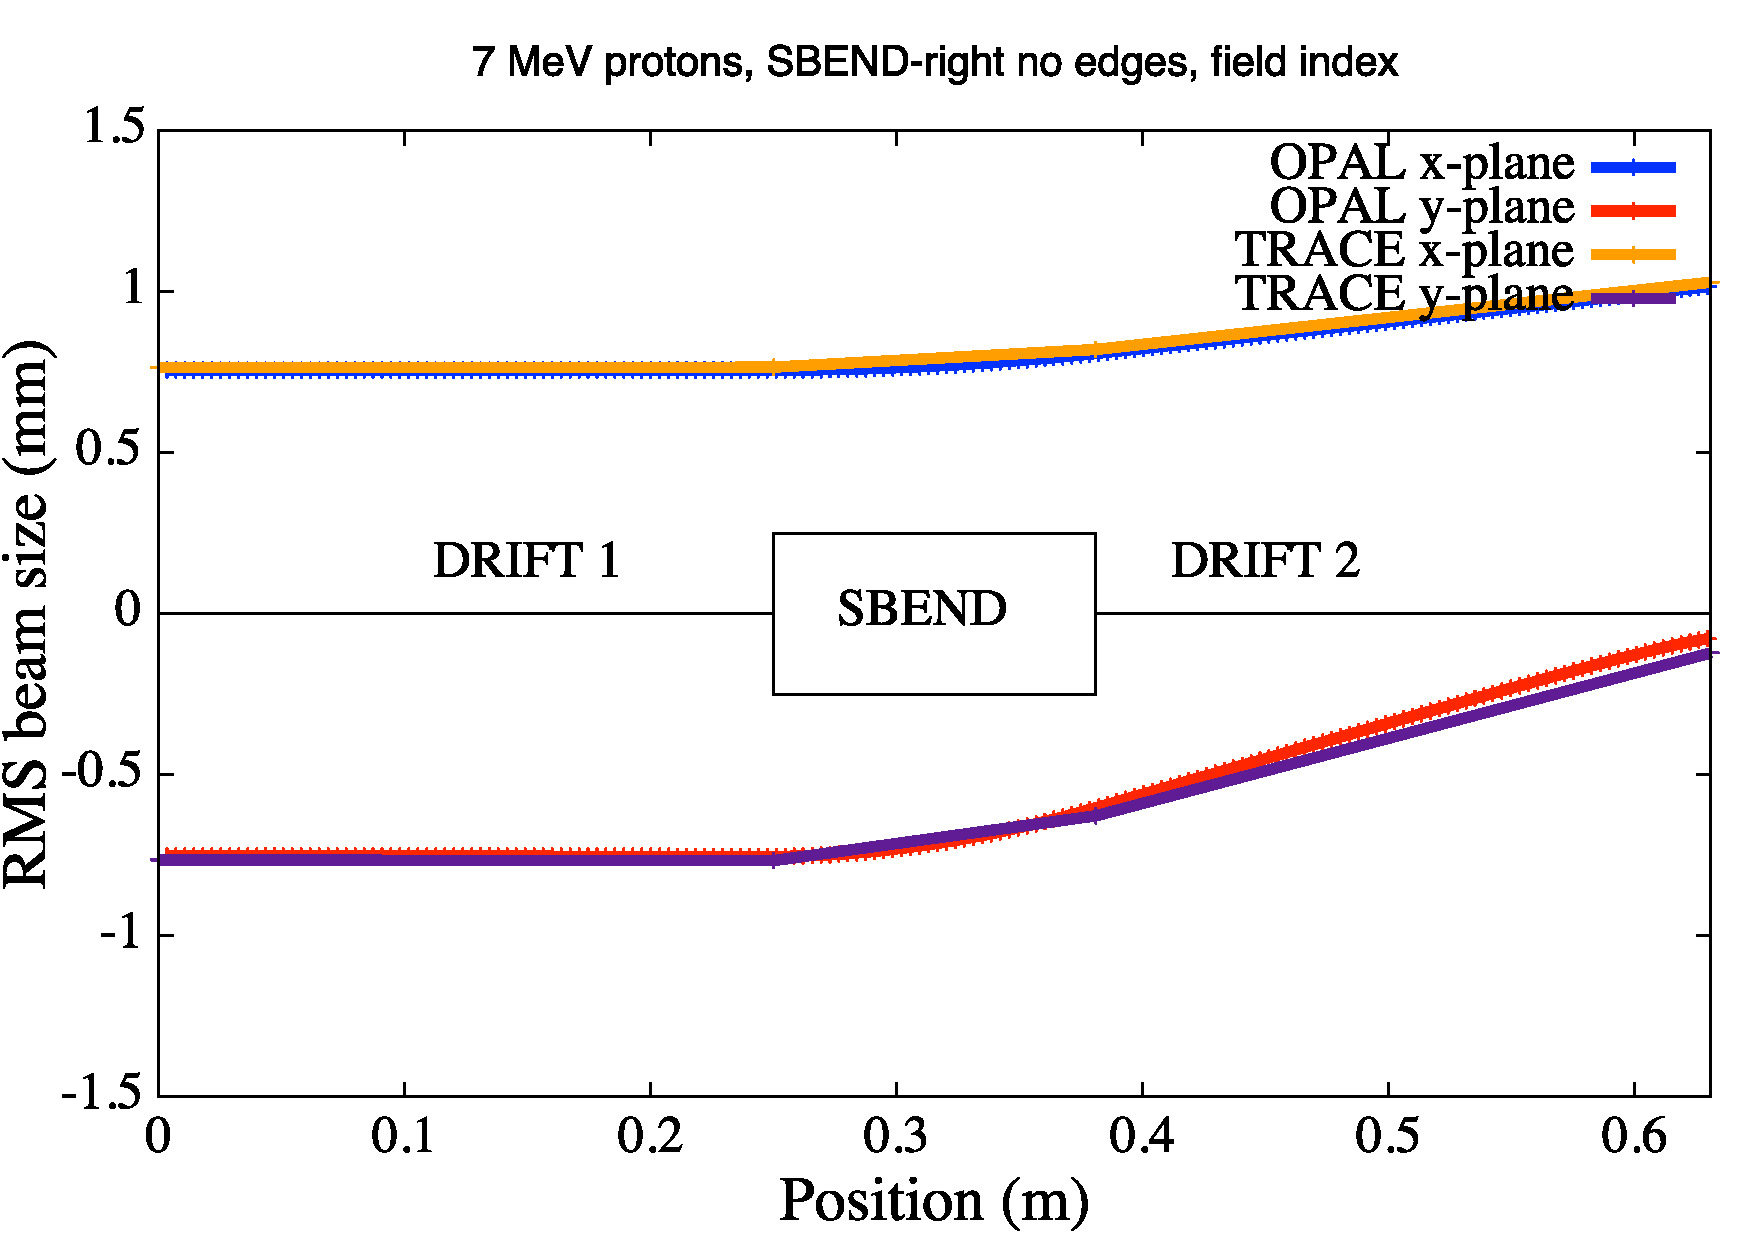
\includegraphics[width=0.5\textwidth-1cm, keepaspectratio=true]{figures/Benchmarks/FI_SBEND_FMTest_Env_T2.pdf}}
    \hspace{1.8cm}
    \subfloat[Transverse RMS emittance]{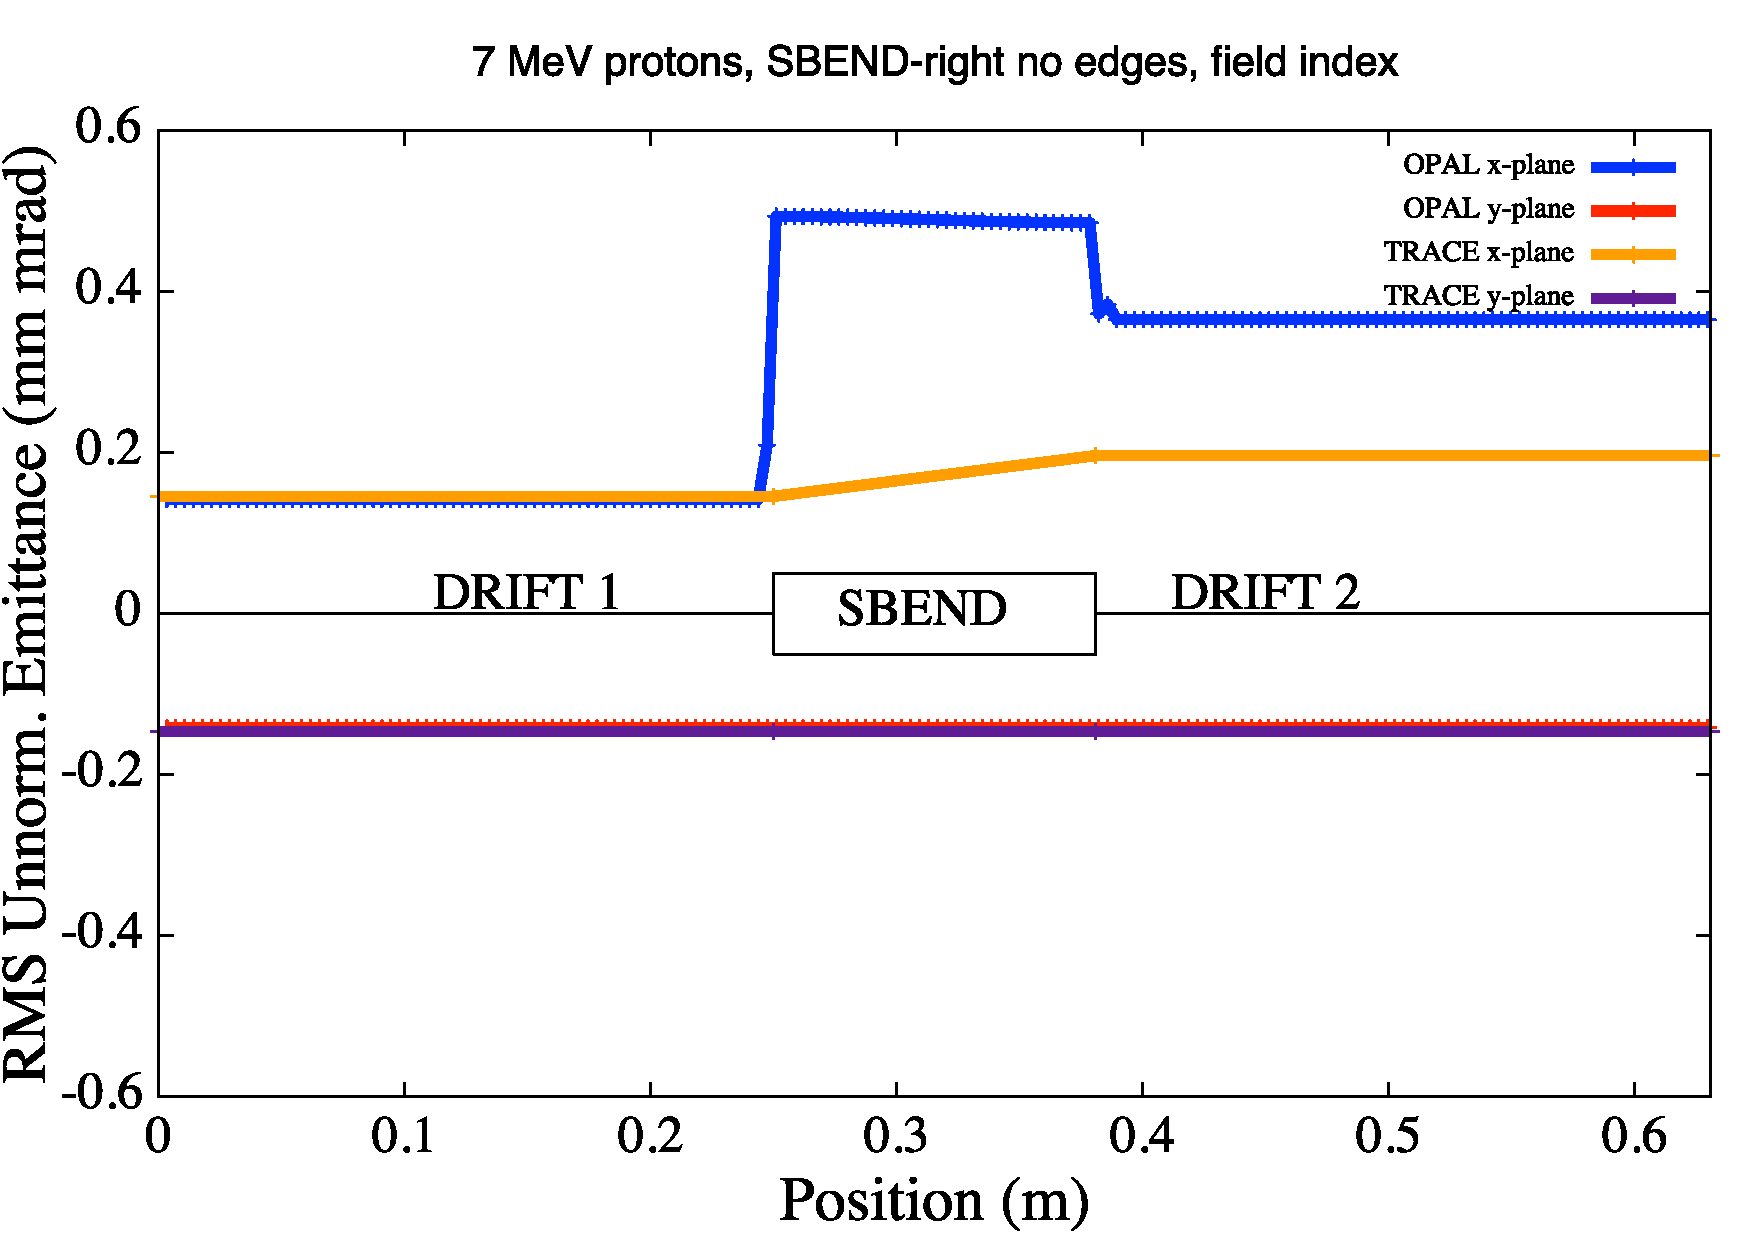
\includegraphics[width=0.5\textwidth-1cm, keepaspectratio=true]{figures/Benchmarks/FI_SBEND_FMTest_Emit_T2.pdf}}
    \caption{TRACE 3D and \opal comparison: SBEND with field index and test field map}
    \label{fig:SBEND_FI_test}
 \end{center}
 \end{figure}
\end{itemize}

\subsubsection{From TRACE 3D to \opalt}
\label{ssec:T3DtoOPAL}

\begin{table}[!ht]
\centering
\caption{Bending magnet features in TRACE 3D and \opalt}
\label{tab:Bend_Trace_OPAL}
     \begin{tabular}{|l|l|l|}
        \hline
        \tabhead{Parameter         & Trace 3D              & \opalt}
        \hline
        \textbf{Bend card}         & 8                     & \keyword{SBEND} or \keyword{RBEND} \\
        Angle                      & Input parameter [deg] & Input/Calc. parameter [rad]        \\
        Magn. field                & Calculated. [T]       & Input/Calc  parameter [T]          \\
        Radius of curv.            & Input parameter [mm]  & Output information [m]             \\
        Field-index                & Input parameter       & Input parameter                    \\
        Length                     & Calculated [mm]       & Input/Calc parameter [m]           \\
        Length type                & Effective             & Straight                           \\
        \hline
        \hline
        \textbf{Edge card}         & 9                     & \keyword{SBEND} or \keyword{RBEND} \\
        Edge angle                 & Input parameter [deg] & Input parameter [rad]              \\
        \hline
        \hline
        \textbf{Vertical gap}      & 9                     & \keyword{SBEND} or \keyword{RBEND} \\
        Gap                        & Total [mm]            & Total [m]                          \\
        \hline
        \hline
        \textbf{Fringe field card} & 9                     & FIELD MAP                          \\
        $K_1$                      & Default: 0.45         & -                                  \\
        $K_2$                      & Default: 2.8          & -                                  \\
        \hline
        \hline
        \textbf{Bend direction}    & Bend angle sign       & Coord. rotation                    \\
        Horiz. right               & Angle $>$ 0           & Angle $>$ 0                        \\
        Horiz. left                & Angle $<$ 0           & Angle $<$ 0                        \\
        Vertical bend              & Card 8, vf $>$ 0      & Coord. rotation                    \\
        \hline
        \end{tabular}
\end{table}

\clearpage

%----------------------------------------------------------------------------------------
% Conclusion
%----------------------------------------------------------------------------------------

\subsection{Conclusion}
\label{sec:conclusion}

\begin{itemize}

\item \textbf{TRACE 3D and TRANSPORT:} \\
- a perfect agreement has been found between these two codes in transversal envelope and emittance; \\
- changing the TRANSPORT units, the input beam parameters, in terms of sigma-matrix coefficients, can directly be imported from TRACE 3D file.

\item \textbf{TRACE 3D and \opalt:} \\
- a good agreement has been found between these two codes in case of sector bending magnet with and without edge angles;\\
% ADA  the field index definition should be clarified according to the results of TEST1, TEST2 and TEST3; \\
- the default magnetic field map seems not working properly if the field index is not zero\\
- an improvement of the test map used is needed in order to match the TRACE 3D emittance \seefig{SBEND_FI_test}.
\end{itemize}


\section{Hard Edge Dipole Comparison with ELEGANT}

\subsection{\opal Dipole}
When defining a dipole (\keyword{SBEND} or \keyword{RBEND}) in \opal,  a fringe field map which defines the range of the field and the Enge coefficients is required. If no map is provided, the code uses a default map. Here is a dipole definition using the default map:

\begin{description}
\item[Example:]
\item \begin{example}
      bend1: SBEND, ANGLE = bend_angle,
      E1 = 0, E2 = 0,
      FMAPFN = "1DPROFILE1-DEFAULT",
      ELEMEDGE = drift_before_bend,
      DESIGNENERGY = bend_energy,
      L = bend_length,
      WAKEF = FS_CSR_WAKE;
      \end{example}
\end{description}
Please refer to \secref{1DProfile1} for the definition of the field map and the default map \keyword{1DPROFILE1-DEFAULT}. It defines a fringe field that extends to 10 cm away from a dipole edge in both directions and it has both $B_y$ and $B_z$ components. This makes the comparison between \opal and other codes which uses a hard edge dipole by default,cumbersome because one needs to carefully integrate thought the fringe field region in \opal in order to come up with the integrated fringe field value (FINT in ELEGANT) that usually used by these codes, e.g. the ELEGANT and the TRACE3D. So we need to find a default map for the hard edge dipole in \opal.

\subsection{Map for Hard Edge Dipole}
The proposed default map for a hard edge dipole can be:
\begin{description}
\item
\begin{example}
1DProfile1  0  0  2
-0.00000001 0.0 0.00000001 3
-0.00000001 0.0 0.00000001 3
-99.9
-99.9
\end{example}
\end{description}
On the first line, the two zeros following  \texttt{1DProfile1} are the orders of the Enge coefficient for the entrance and exit edge of the dipole. $2 cm$ is the default dipole gap width. The second line defines the fringe field region of the entrance edge of the dipole which extends from $-0.00000001 cm$ to $0.00000001 cm$.  The third line defines the same fringe field region for the exit edge of the dipole. The $3$s on both line don't mean anything, they are just placeholders. On the fourth and fifth line, the zeroth order Enge coefficients for both edges are given. Since they are large negative numbers, the field in the fringe field region has no $B_z$ component and its $B_y$ component is just like the field in the middle of the dipole.
\begin{figure}[!htbp]
\centering
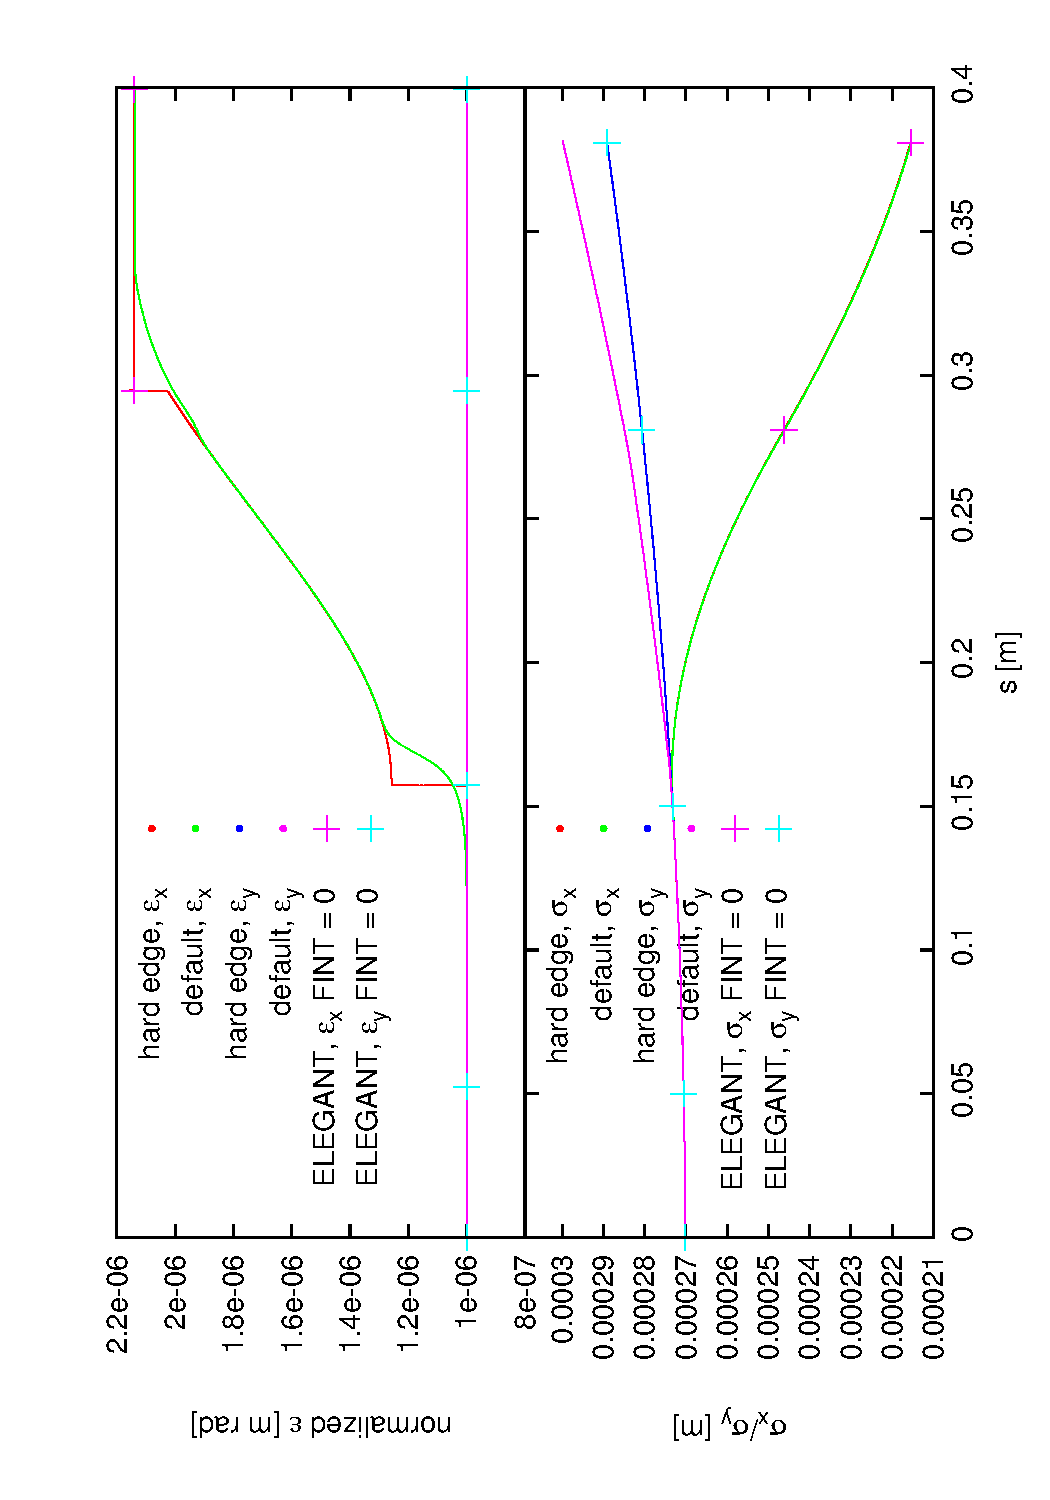
\includegraphics[height=0.5\textwidth-0.6cm, angle = -90, trim = 8mm 10mm 2mm 10mm, clip]{figures/Benchmarks/report-compare-default}
\caption{Compare emittances and beam sizes obtained by using the hard edge map (\opal), the default map (\opal), and the ELEGANT}
\label{fig:plot-compare-default}
\end{figure}
\figref{plot-compare-default} compares the emittances and beam sizes obtained by using the hard edge map, the default map and the ELEGANT. One can see that the results produced by the hard edge map match the ELEGANT results when FINT is set to zero.

\subsection{Integration Time Step}
When the hard edge map is used for a dipole, finer integration time step is needed to ensure the accurate of the calculation. \figref{plot-emit-dt} compares the normalized emittances generated using the hard edge map in \opal with varying time steps to those from the ELEGANT. \SI{0.01}{\pico\second} seems to be a optimal time step for the fringe field region. To speed up the simulations, one can use larger time steps outside the fringe field regions. In \figref{plot-emit-dt}, one can observe a discontinuity in the horizontal emittance when the hard edge map is used in the calculation. This discontinuity comes from the fact that \opal emittance is calculated at an instant time. Once the beam or part of the beam gets into the dipole, its $P_x$ gets a kick which will result in a sudden emittance change.
\begin{figure}[!htbp]
\centering
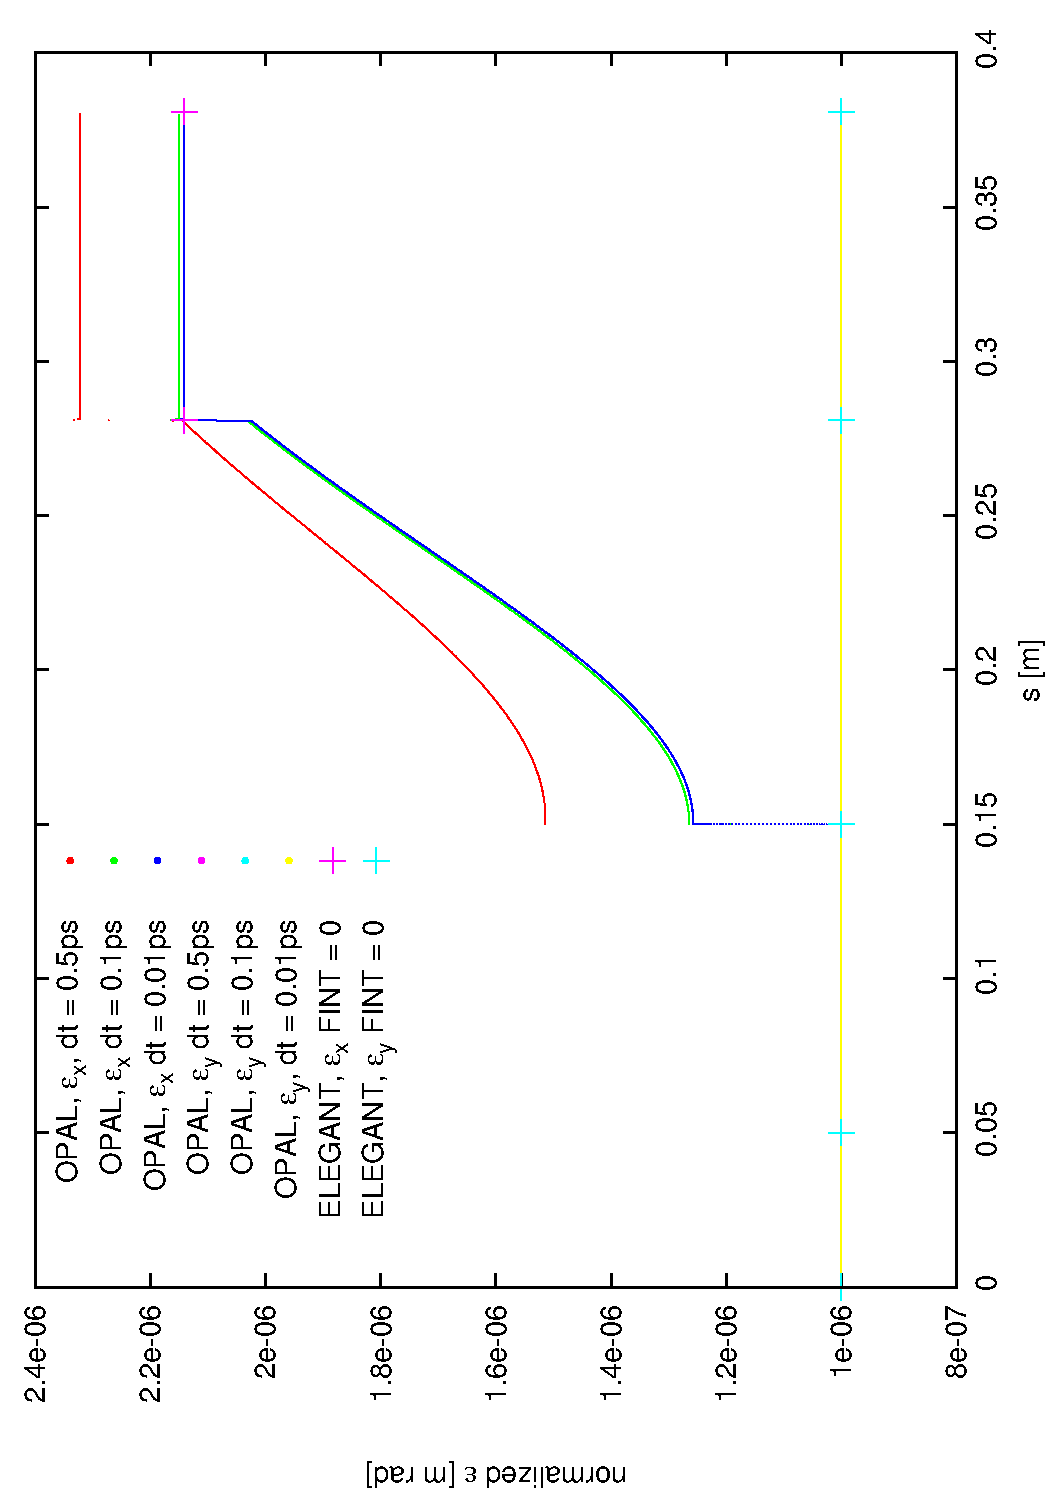
\includegraphics[width=0.5\textwidth-0.6cm,
%angle = -90,
trim = 20mm 0mm 8mm 0mm, clip]{figures/Benchmarks/report-emit-dt}
\caption{Horizontal and vertical normalized emittances for different integration time steps}
\label{fig:plot-emit-dt}
\end{figure}

\figref{plot-fringe-size,plot-fringe-size-zoom} examine the effects of the fringe field range and the integration time step on the simulation accuracy. \figref{plot-fringe-size-zoom} is a zoom-in plot of \figref{plot-fringe-size}. We can conclude that the size of the integration time step has more influence on the accuracy of the simulation.
\begin{figure}[!htbp]
\centering
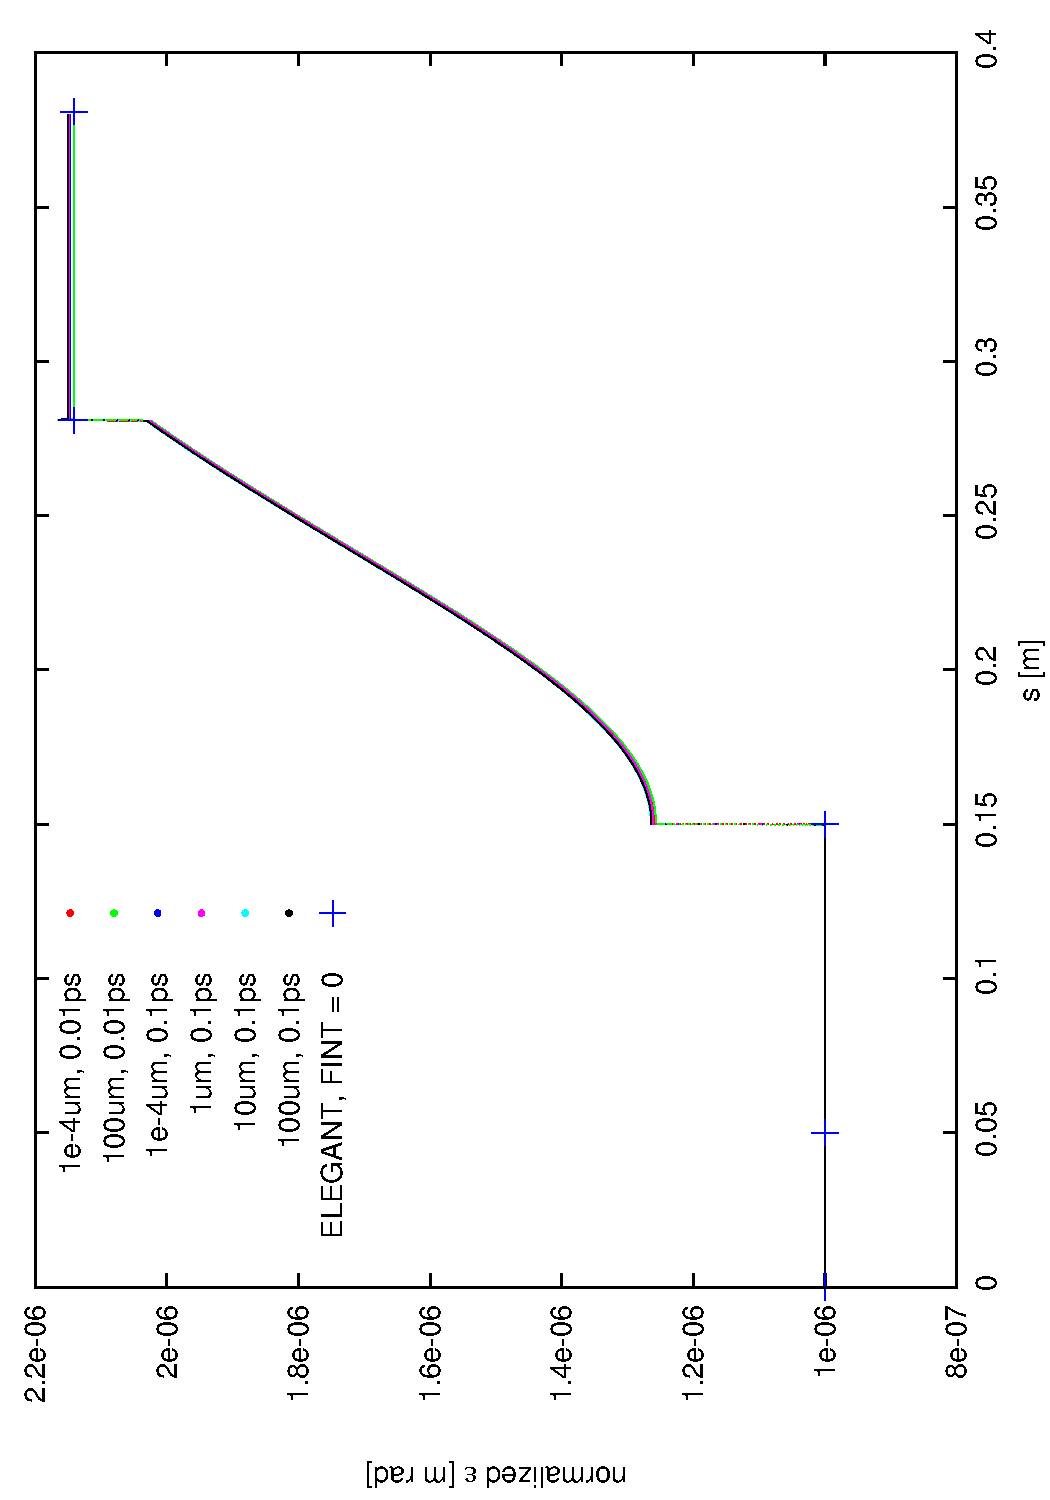
\includegraphics[height=0.5\textwidth-0.6cm, angle = -90, trim = 3mm 0mm 2mm 0mm, clip]{figures/Benchmarks/report-fringe-size}
\caption{Normalized horizontal emittance for different fringe field ranges and integration time steps}
\label{fig:plot-fringe-size}
\end{figure}
\begin{figure}[!htbp]
\centering
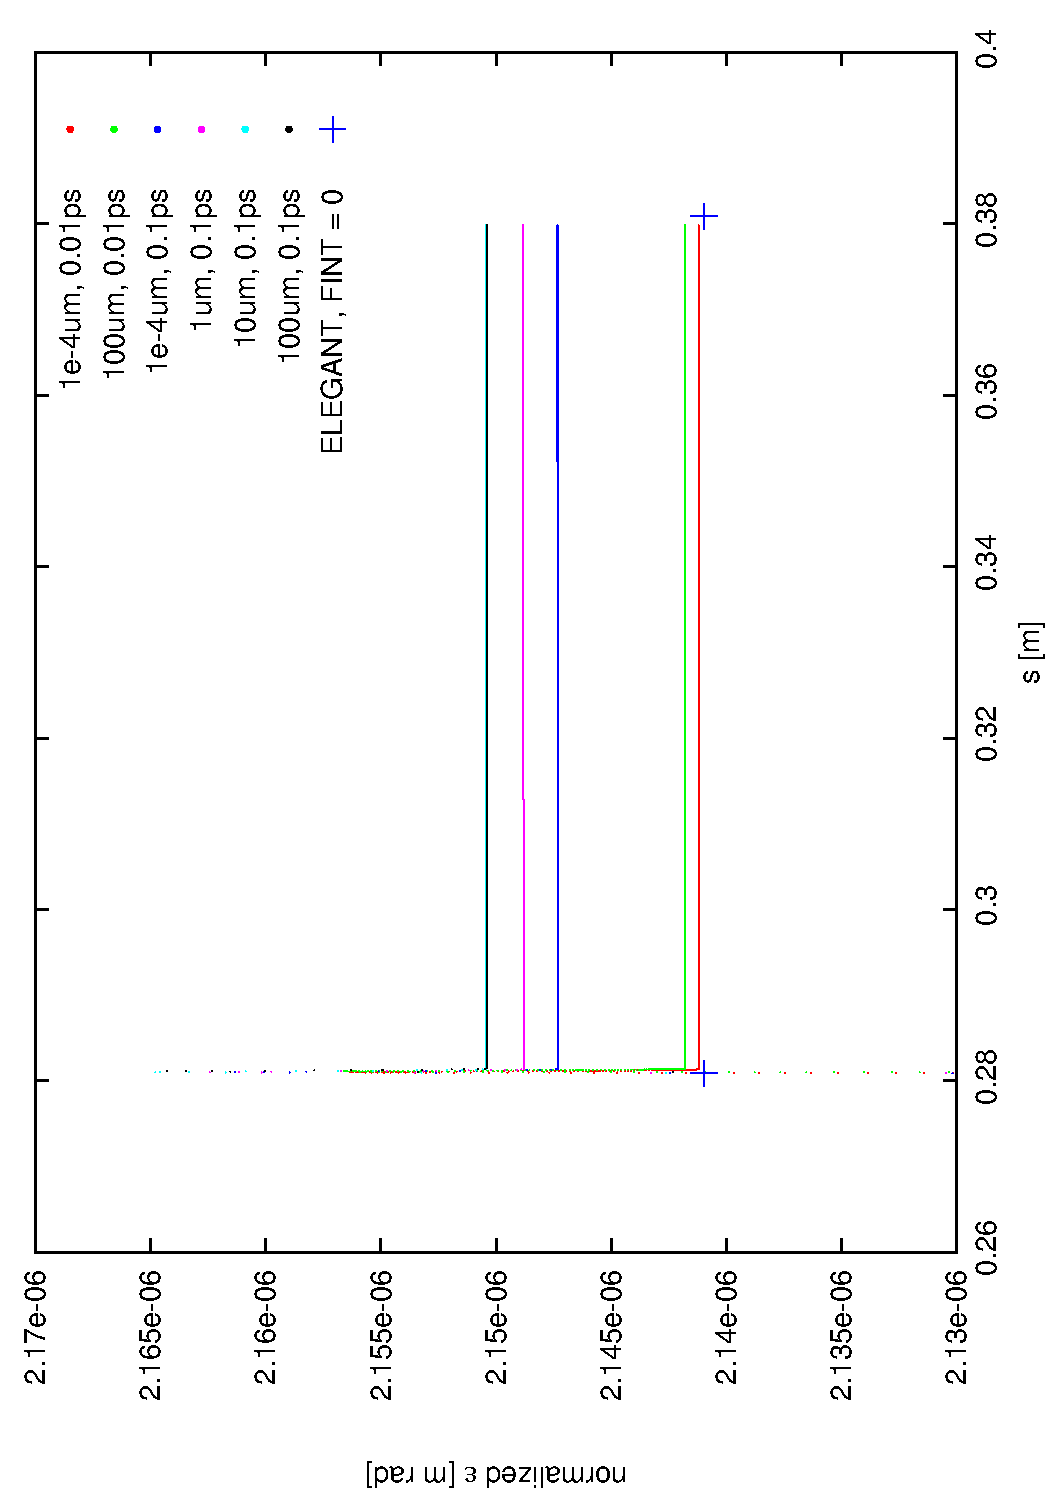
\includegraphics[height=0.5\textwidth-0.6cm, angle = -90, trim = 3mm 0mm 2mm 0mm, clip]{figures/Benchmarks/report-fringe-size-zoom}
\caption{Zoom in on the final emittance in \figref{plot-fringe-size-zoom}}
\label{fig:plot-fringe-size-zoom}
\end{figure}

\section{1D CSR comparison with ELEGANT}
1D-CSR wake function can now be used for the drift element by defining its attribute \keyword{WAKEF = FS\_CSR\_WAKE}. In order to calculate the CSR effect correctly, the drift has to follow a bending magnet whose CSR calculation is also turned on.

\begin{description}
\item[Example:]
\item \begin{example}
      bend1: SBEND, ANGLE = bend_angle,
      E1 = 0, E2 = 0,
      FMAPFN = ``1DPROFILE1-DEFAULT'',
      ELEMEDGE = drift_before_bend,
      DESIGNENERGY = bend_energy,
      L = bend_length,
      WAKEF = FS_CSR_WAKE;
      \end{example}
\item  \begin{example}
       drift1: DRIFT, L=0.4, ELEMEDGE = drift_before_bend +
       bend_length, WAKEF = FS_CSR_WAKE;
       \end{example}
\end{description}

\subsection{Benchmark}
The \opal dipoles all have fringe fields. When comparisons are done between \opal and ELEGANT \cite{elegant} for example, one needs to appropriately set the FINT attribute of the bending magnet in ELEGANT in order to represent the field correctly. Although ELEGANT tracks in the ($x, x', y, y', s, \delta$) phase space, where $\delta = \frac{\Delta p}{p_0}$ and $p_0$ is the momentum of the reference particle, the watch point output beam distributions from the ELEGANT are list in ($x, x', y, y', t, \beta\gamma$). If one wants to compare ELEGANT watch point output distribution to \opal, unit conversion needs to be performed, i.e.
\begin{eqnarray*}
P_x &=& x'\beta\gamma, \\ P_y &=& y'\beta\gamma, \\ s &=& (\bar t-t)\beta c .
\end{eqnarray*}


To benchmark the CSR effect, we set up a simple beamline with 0.1m drift $+$ 30 degree sbend $+$ 0.4m drift. When the CSR effect is turn off, \figref{plot-emit-csr-off} shows that the normalized emittances calculated using both \opal and ELEGANT agree. The emittance values from \opal are obtained from the {\it .stat} file, while for ELEGANT, the transverse emittances are obtained from the sigma output file (enx, and eny), the longitudinal emittance is calculated using the watch point beam distribution output.
\begin{figure}[!htbp]
\centering
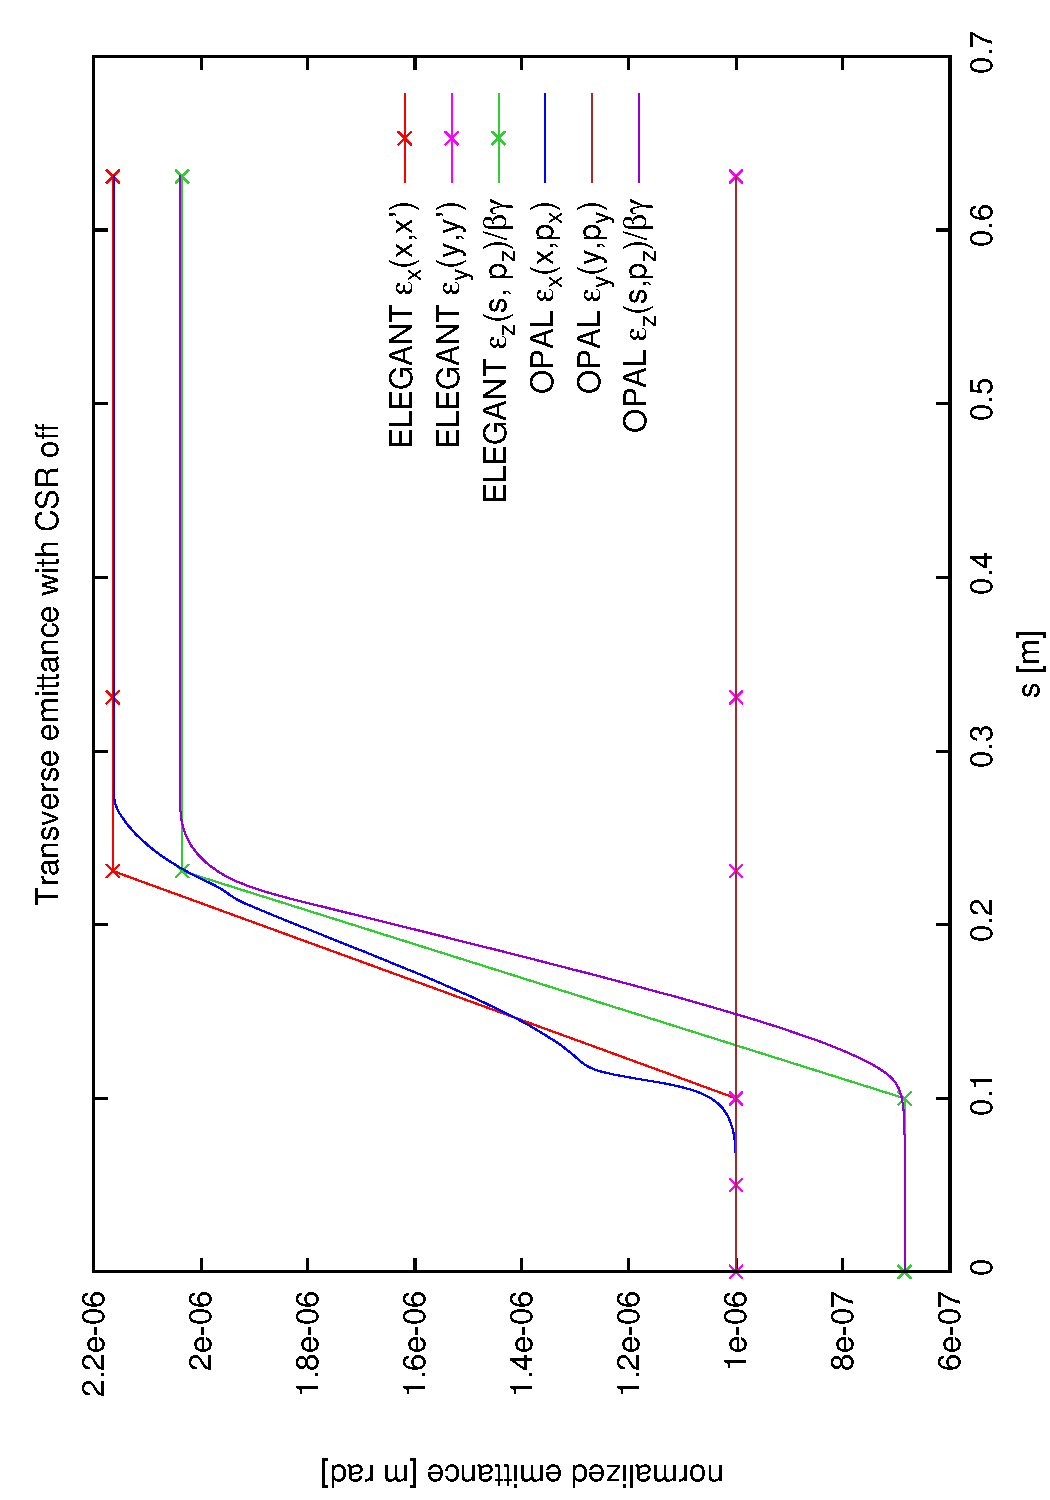
\includegraphics[height=0.5\textwidth-0.6cm, angle = -90, trim = 3mm 0mm 2mm 0mm, clip]{figures/Benchmarks/emit-csr-off}
\caption{Comparison of the trace space using ELEGANT and \opal}
\label{fig:plot-emit-csr-off}
\end{figure}

When CSR calculations are enabled for both the bending magnet and the following drift, \figref{plot-dpp-csr-on} shows the average $\delta$ or $\frac{\Delta p}{p}$ change along the beam line, and \figref{plot-emit-csr-on} compares the normalized transverse and longitudinal emittances obtained by these two codes. The average $\frac{\Delta p}{p}$ can be found in the centroid output file (Cdelta) from ELEGANT, while in \opal, one can calculate it using $\frac{\Delta p}{p} = \frac{1}{\beta^2}\frac{\Delta \overline{E}}{\overline{E}+mc^2}$, where $\Delta \overline{E}$ is the average kinetic energy from the {\it .stat} output file.
\begin{figure}[!htbp]
\centering
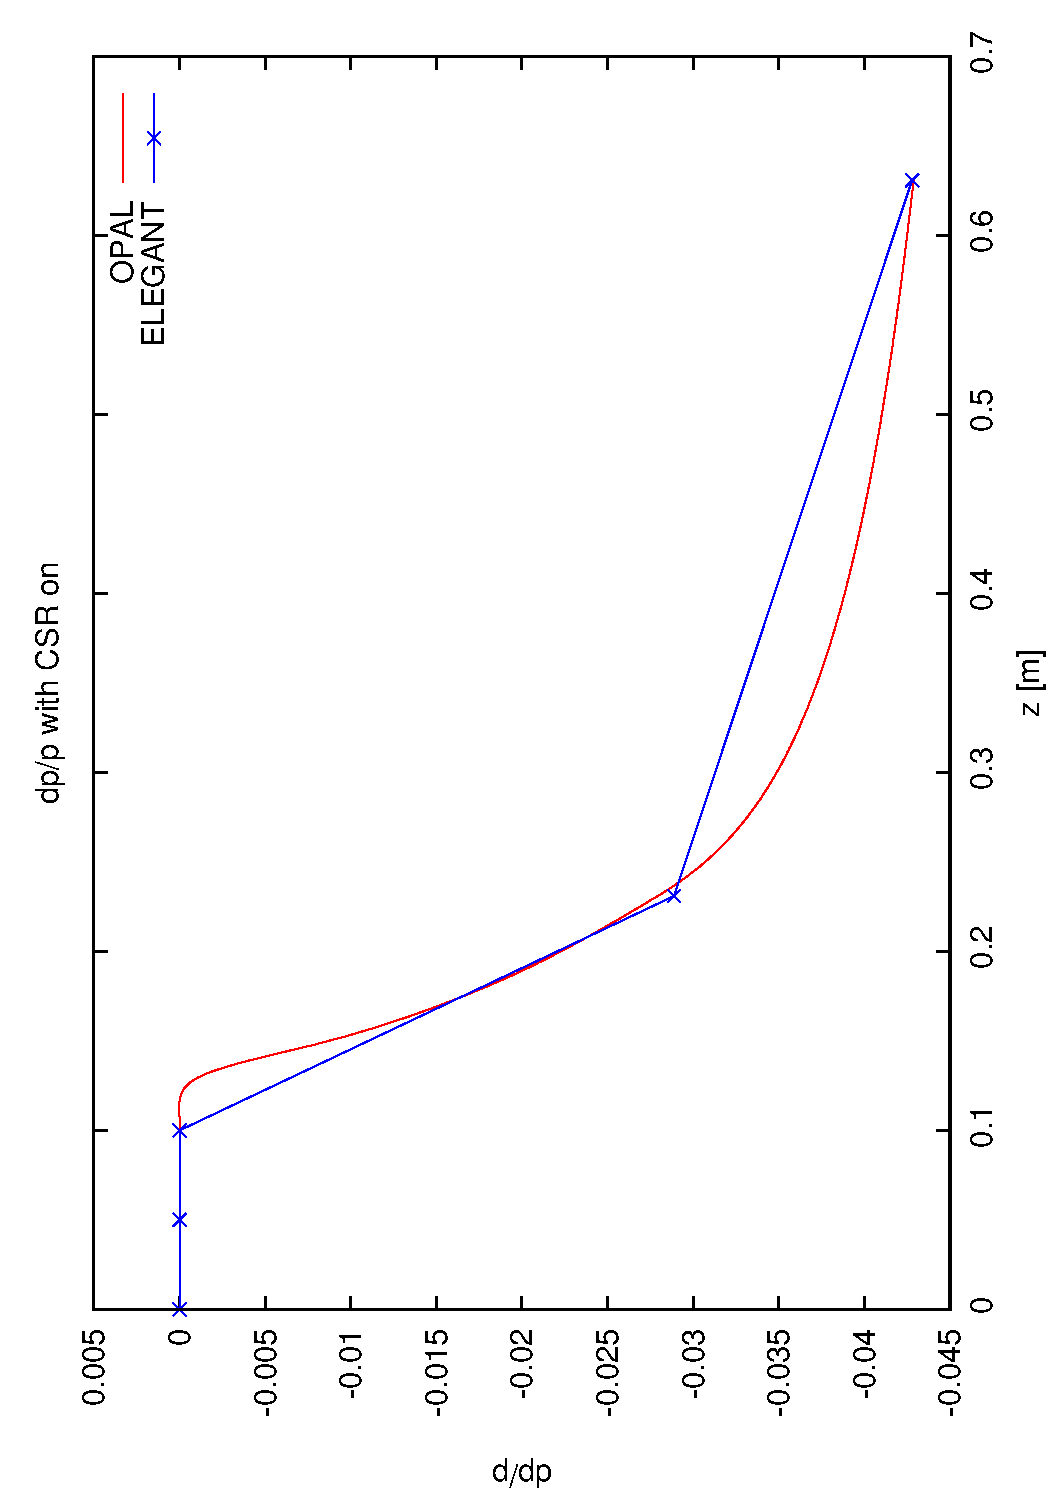
\includegraphics[height=0.5\textwidth-0.6cm, angle = -90, trim = 3mm 0mm 2mm 0mm, clip]{figures/Benchmarks/dpp-csr-on}
\caption{$\frac{\Delta p}{p}$ in Elegant and \opal}
\label{fig:plot-dpp-csr-on}
\end{figure}
In the drift space following the bending magnet, the CSR effects are calculated using Stupakov's algorithm with the same setting in both codes. The average fractional momentum change $\frac{\Delta p}{p}$ and the longitudinal emittance show good agreements between these codes. However, they produce different horizontal emittances as indicated in \figref{plot-emit-csr-on}.
\begin{figure}[!htbp]
\centering
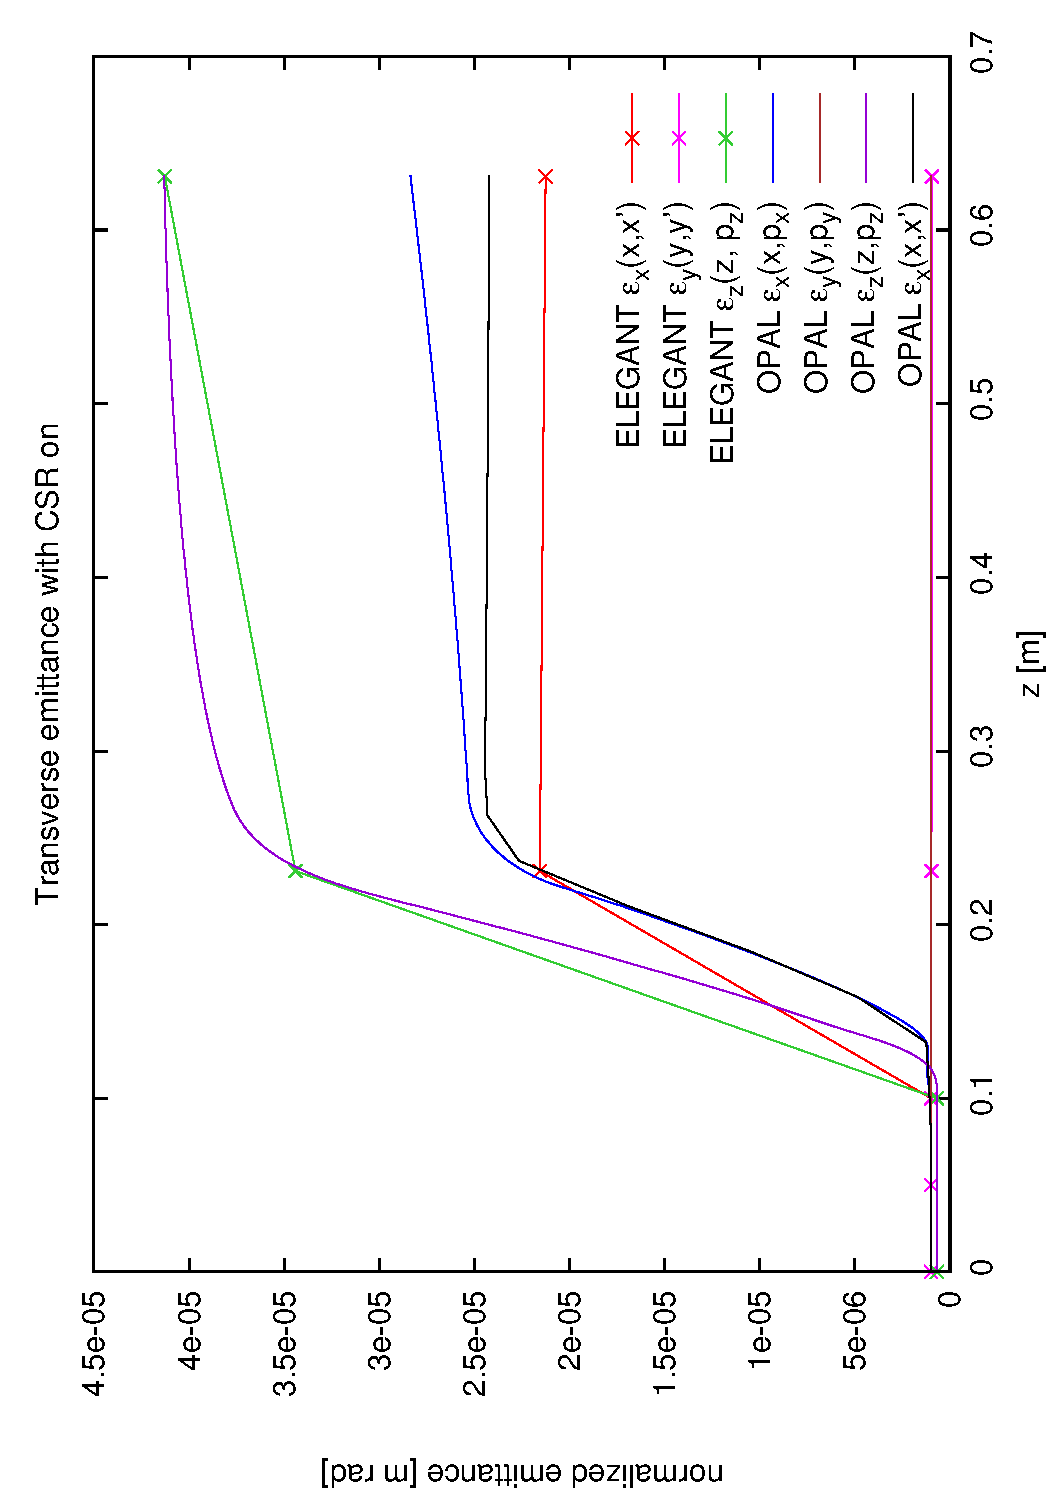
\includegraphics[height=0.5\textwidth-0.6cm, angle = -90, trim = 3mm 0mm 2mm 0mm, clip]{figures/Benchmarks/emit-csr-on}
\caption{Transverse emittances in ELEGANT and \opal}
\label{fig:plot-emit-csr-on}
\end{figure}

One important effect to notice is that in the drift space following the bending magnet, the normalized emittance $\epsilon_x(x, P_x)$ output by \opal keeps increasing while the trace-like emittance $\epsilon_x(x, x')$ calculated by ELEGANT does not. This can be explained by the fact that with a relatively large energy spread (about $3\%$ at the end of the dipole due to CSR), {\bf an correlation} between transverse position and energy can build up in a drift thereby induce emittance growth. However, this effect can only be observed in the normalized emittance calculated with $\epsilon_x(x, P_x) = \sqrt{\langle x^2 \rangle \langle P_x^2\rangle - \langle xP_x \rangle^2}$ where $P_x = \beta\gamma x'$, not the trace-like emittance which is calculated as $\epsilon_x(x, x') = \beta\gamma\sqrt{\langle x^2 \rangle \langle x'^2 \rangle - \langle xx' \rangle^2}$ \cite{prstab2003}. In \figref{plot-emit-csr-on}, a trace-like horizontal emittance is also calcualted for the \opal output beam distributions. Like the ELEGANT result, this trace-like emittance doesn't grow in the drift. However, their differences come from the ELEGANT's lack of CSR effect in the fringe field region.

\section{\opal \& \impactt}
This benchmark compares rms quantities such as beam size and emittance of \opal and \impactt \cite{qiang2005, qiang2006-1, qiang2006-2}. A {\bf cold} \SI{10}{\milli\ampere} H+ bunch is expanding in a \SI{1}{\meter} drift space. A Gaussian distribution, with a cut at 4 $\sigma$ is used. The charge is computed by assuming a \SI{1}{\mega\hertz} structure i.e. $Q_{\text{tot}}=\frac{I}{\nu_{\text{rf}}}$. For the simulation we use a grid with $16^{3}$ grid point and open boundary condition. The number of macro
particles is $N_{\text{p}} = 10^{5}$.

\subsection{\opal Input}
\begin{longexample}
OPTION, ECHO = FALSE, PSDUMPFREQ = 10,
STATDUMPFREQ = 10, REPARTFREQ = 1000,
PSDUMPLOCALFRAME = FALSE;

TITLE, string="Gaussian bunch drift test";

Edes    = 0.001;        // GeV
CURRENT = 0.01;  // A

gamma=(Edes+PMASS)/PMASS;
beta=sqrt(1-(1/gamma^2));
gambet=gamma*beta;
P0 = gamma*beta*PMASS;

D1: DRIFT, ELEMEDGE = 0.0, L = 1.0;

L1: LINE = (D1);

Fs1: FIELDSOLVER, FSTYPE = FFT, MX = 16, MY = 16, MT = 16, BBOXINCR=0.1;

Dist1: DISTRIBUTION, DISTRIBUTION = GAUSS,
       OFFSETX = 0.0, OFFSETY = 0.0, OFFSETZ = 15.0e-3,
       SIGMAX = 5.0e-3, SIGMAY = 5.0e-3, SIGMAZ = 5.0e-3,
       OFFSETPX = 0.0, OFFSETPY = 0.0, OFFSETPZ = 0.0,
       SIGMAPX = 0.0 , SIGMAPY = 0.0 , SIGMAPZ = 0.0 ,
       CORRX = 0.0, CORRY = 0.0, CORRZ = 0.0,
       CUTOFFX = 4.0, CUTOFFY = 4.0, CUTOFFLONG = 4.0;

Beam1: BEAM, PARTICLE = PROTON, CHARGE = 1.0, BFREQ = 1.0e6, PC = P0,
               NPART = 1E5, BCURRENT = CURRENT, FIELDSOLVER = Fs1;

SELECT, LINE = L1;

TRACK, LINE = L1, BEAM = Beam1, MAXSTEPS = 1000, ZSTOP = 1.0, DT = 1.0e-10;
 RUN, METHOD = "PARALLEL-T", BEAM = Beam1, FIELDSOLVER = Fs1, DISTRIBUTION = Dist1;
ENDTRACK;
STOP;
\end{longexample}

\subsection{\impactt Input}
\begin{longexample}
!Welcome to \impactt input file.
!All comment lines start with "!" as the first character of the line.
! col row
1 1
!
! information needed by the integrator:
! step-size, number of steps, and number of bunches/bins (??)
!
!   dt    Ntstep  Nbunch
1.0e-10   700     1
!
! phase-space dimension, number of particles, a series of flags
! that set the type of integrator, error study, diagnostics, and
! image charge, and the cutoff distance for the image charge
!
! PSdim  Nptcl   integF  errF  diagF  imchgF  imgCutOff (m)
6 100000  1 0 1 0 0.016
!
! information about mesh: number of points in x, y, and z, type
! of boundary conditions, transverse aperture size (m),
! and longitudinal domain size (m)
!
!  Nx  Ny  Nz  bcF   Rx    Ry    Lz
16 16 16 1 0.15 0.15 1.0e5
!
!
! distribution type number (2 == Gauss), restart flag, space-charge substep
! flag, number of emission steps, and max emission time
!
! distType  restartF  substepF  Nemission  Temission
2           0         0         -1          0.0
!
!  sig*   sigp*  mu*p*  *scale  p*scale  xmu*      xmu*
!
0.005 0.0 0.0  1. 1. 0.0 0.0
0.005 0.0 0.0  1. 1. 0.0 0.0
0.005 0.0 0.0  1. 1. 0.0 0.0462
!
! information about the beam: current, kinetic energy, particle
! rest energy, particle charge, scale frequency, and initial cavity phase
!
! I/A   Ek/eV     Mc2/eV          Q/e  freq/Hz  phs/rad
0.010   1.0e6     938.271998e+06  1.0  1.0e6      0.0
!
!
! ======= machine description starts here =======
! the following lines, which must each be terminated with a '/',
! describe one beam-line element per line; the basic structure is
! element length, ???, ???, element type, and then a sequence of
! at most 24 numbers describing the element properties
!   0  drift tube    2      zedge radius
!   1  quadrupole    9      zedge, quad grad, fileID,
!                             radius, alignment error x, y
!                             rotation error x, y, z
! L/m  N/A N/A  type  location of starting edge  v1  <B0><B0><B0>  v23 /
1.0    0   0    0    0.0                           0.5            /
\end{longexample}

\subsection{Results}
A good agreement is shown in the \figref{plot-opal-impact1,plot-opal-impact2}. This proves to some extend the compatibility of the
space charge solvers of \opal and \impactt.

\begin{figure}[!htbp]
\centering
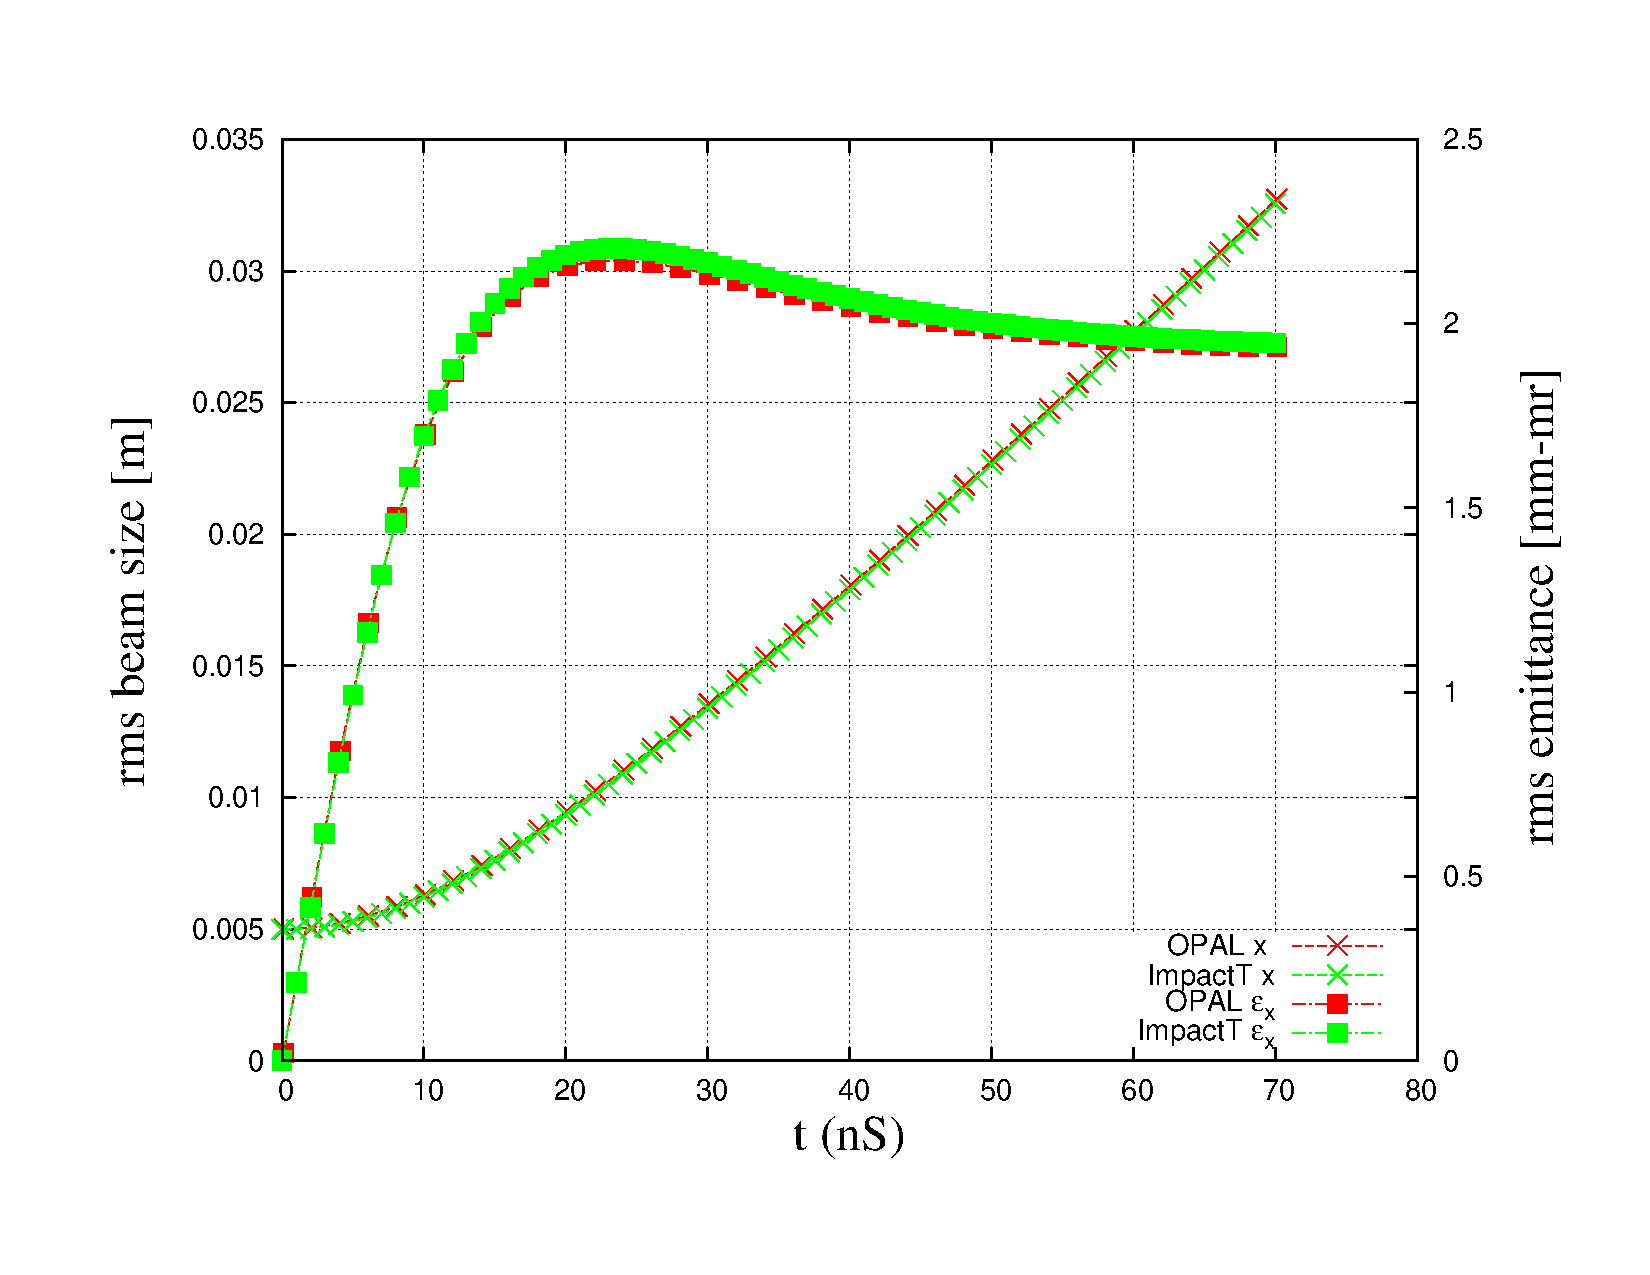
\includegraphics[width=0.5\textwidth-0.6cm, angle = 0, trim = 20mm 0mm 15mm 0mm, clip]{figures/Benchmarks/opal-impact-1MHz-x}
\hspace{1cm}
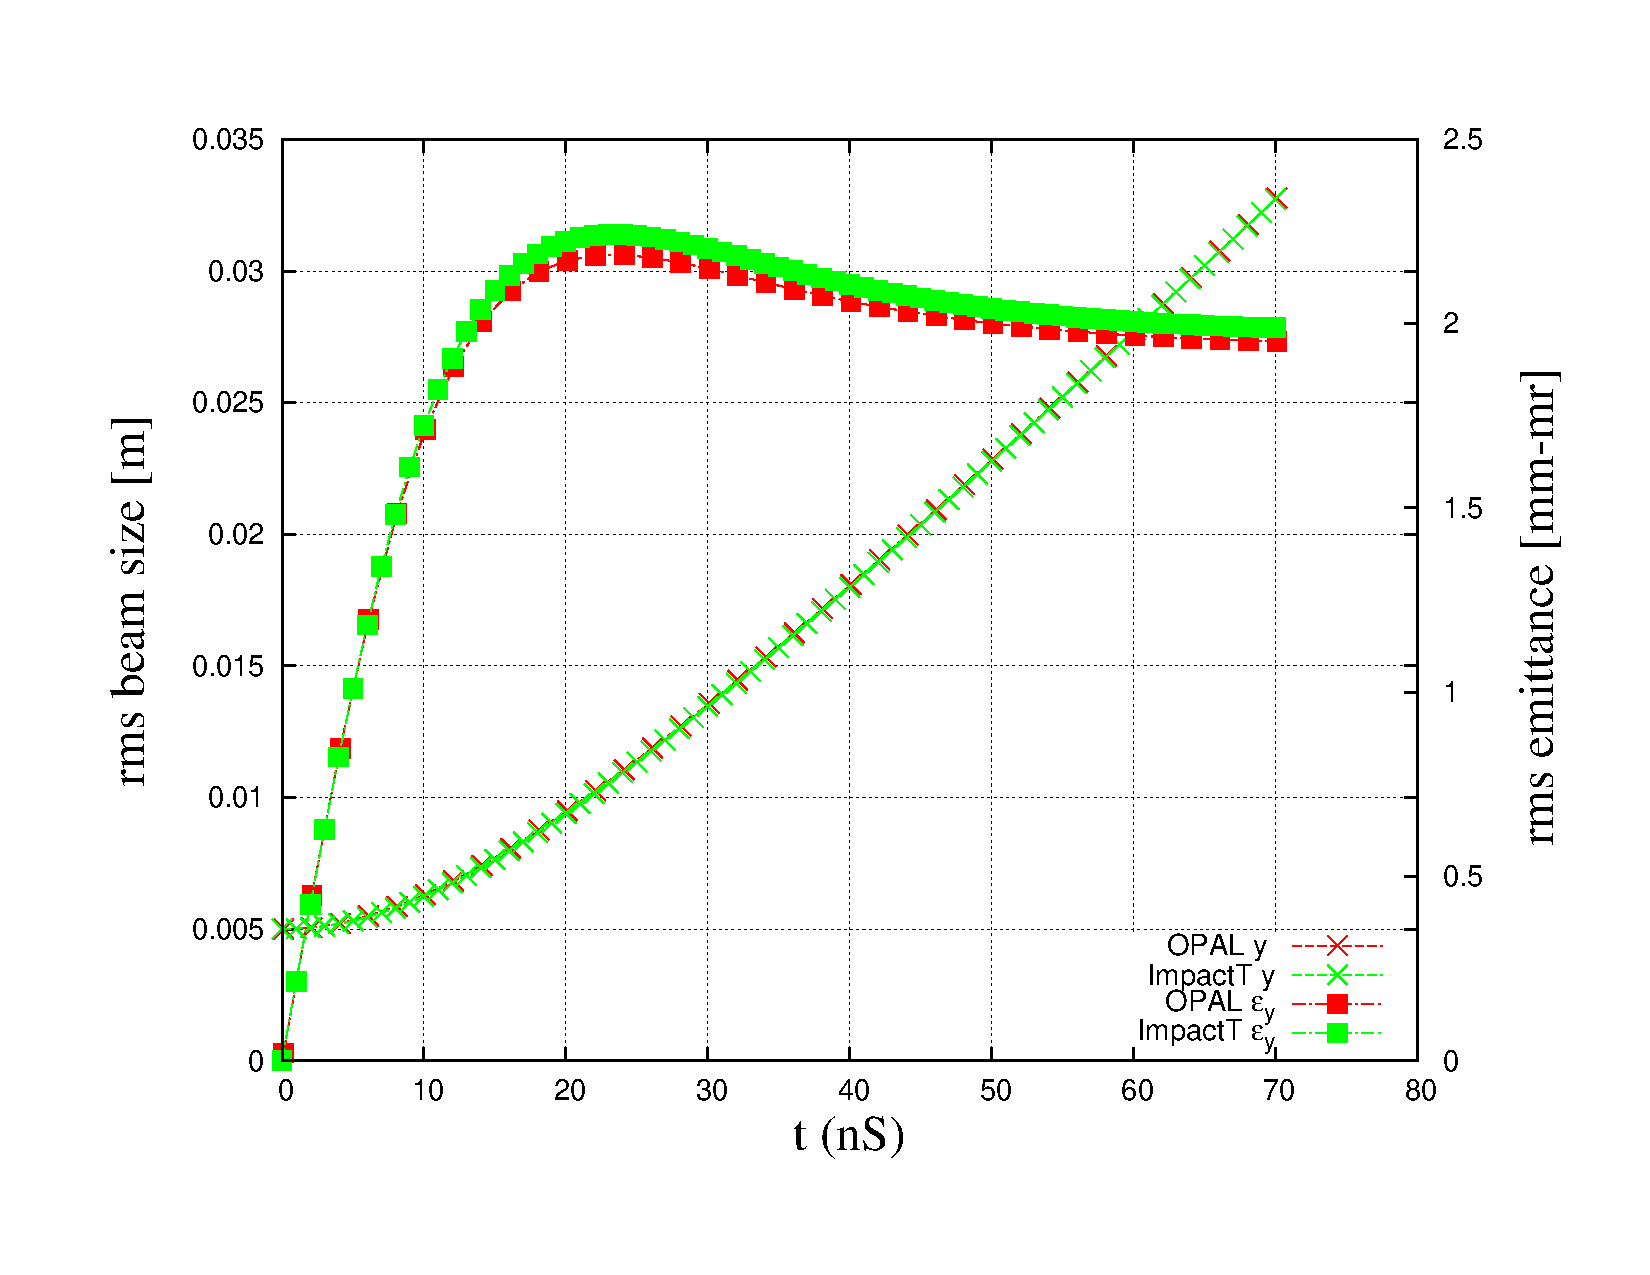
\includegraphics[width=0.5\textwidth-0.6cm, angle = 0, trim = 20mm 0mm 15mm 0mm, clip]{figures/Benchmarks/opal-impact-1MHz-y}
\caption{Transverse beam sizes and emittances in \impactt and \opal}
\label{fig:plot-opal-impact1}
\end{figure}

\begin{figure}[!htbp]
\centering
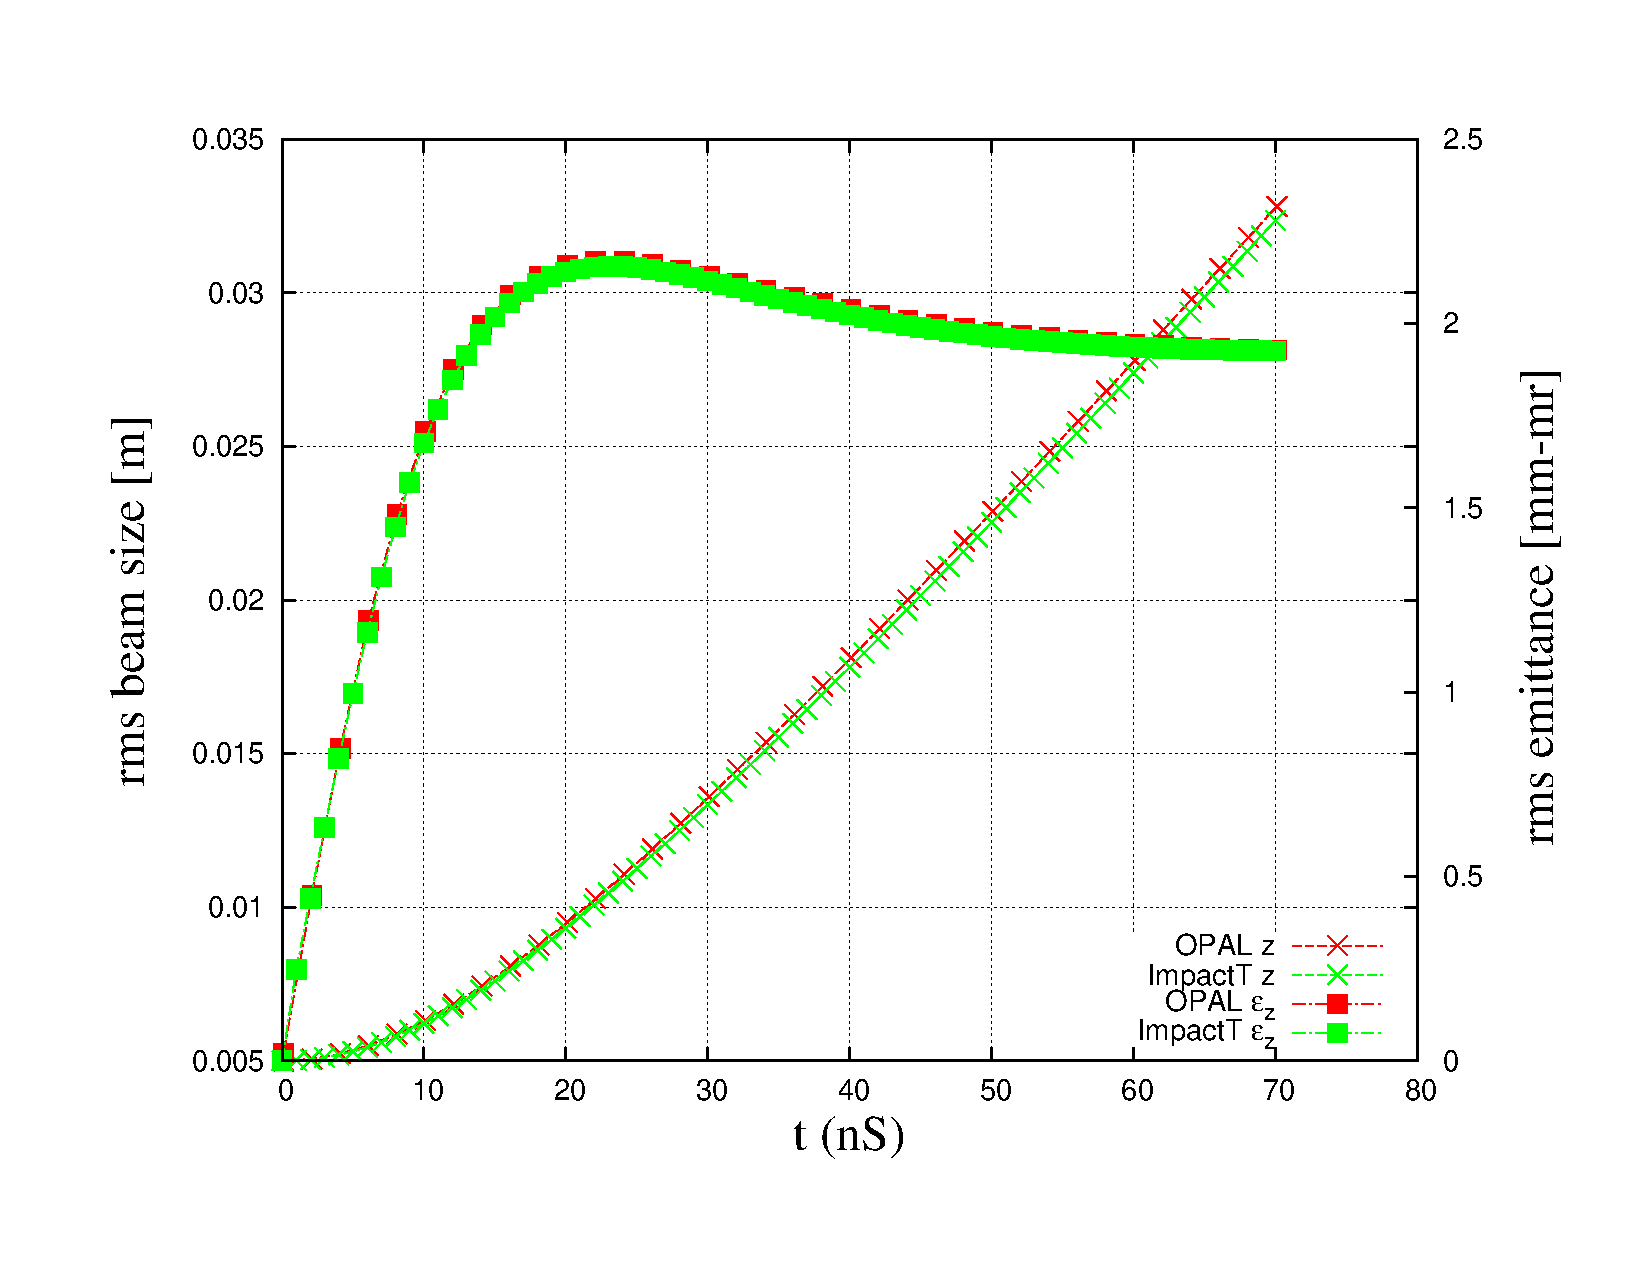
\includegraphics[width=0.5\textwidth-0.6cm, angle = 0, trim = 20mm 0mm 15mm 0mm, clip]{figures/Benchmarks/opal-impact-1MHz-z}
\caption{Longitudinal beam size and emittance in \impactt and \opal}
\label{fig:plot-opal-impact2}
\end{figure}

%----------- Footer control ------------------
\ifthenelse{\boolean{FullOPALManual}}
{
  %do nothing
}
% else (for individual document creation)
{
\appendix
\printbibliography
\end{document}
}
%---------------------------------------------